\everymath{\displaystyle}
\documentclass{beamer}
% \documentclass[handout]{beamer}

%\usepackage[pdftex]{color,graphicx}
\usepackage{amsmath,amssymb,amsfonts}

\mode<presentation>
{
  % \usetheme{Darmstadt}
  % \usetheme[hideothersubsections]{Hannover}
  % \usetheme[hideothersubsections]{Goettingen}
  \usetheme[hideothersubsections, right]{Berkeley}

  \usecolortheme{seahorse}
  % \usecolortheme{dolphin}
  \usecolortheme{rose}
  % \usecolortheme{orchid}

  \useinnertheme[shadow]{rounded}

  % \setbeamercovered{transparent}
  \setbeamercovered{invisible}
  % or whatever (possibly just delete it)
}

\mode<handout>{
  \setbeamercolor{background canvas}{bg=black!5}
  \usepackage{pgfpages}
  \pgfpagesuselayout{4 on 1}[a4paper,border shrink=5mm, landscape]
}

\usepackage[brazilian]{babel}
% or whatever

% \usepackage[latin1]{inputenc}
\usepackage[utf8]{inputenc}
% or whatever

\usepackage{times}
%\usepackage[T1]{fontenc}
% Or whatever. Note that the encoding and the font should match. If T1
% does not look nice, try deleting the line with the fontenc.


\title%[] % (optional, use only with long paper titles)
{}

\subtitle
{} % (optional)

\author%[] % (optional, use only with lots of authors)
{Felipe Figueiredo}% \and S.~Another\inst{2}}
% - Use the \inst{?} command only if the authors have different
%   affiliation.

\institute[INTO] % (optional, but mostly needed)
{
}
  % \inst{1}%
  % Department of Computer Science\\
  % University of Somewhere
  % \and
  % \inst{2}%
  % Department of Theoretical Philosophy\\
  % University of Elsewhere}
% - Use the \inst command only if there are several affiliations.
% - Keep it simple, no one is interested in your street address.

\date%[] % (optional)
{}

% \subject{Talks}
% This is only inserted into the PDF information catalog. Can be left
% out. 



% If you have a file called "university-logo-filename.xxx", where xxx
% is a graphic format that can be processed by latex or pdflatex,
% resp., then you can add a logo as follows:

\pgfdeclareimage[height=1.6cm]{university-logo}{../logo}
\logo{\pgfuseimage{university-logo}}



% Delete this, if you do not want the table of contents to pop up at
% the beginning of each subsection:
\AtBeginSubsection[]
%\AtBeginSection[]
{
  \begin{frame}<beamer>{Sumário}
    \tableofcontents[currentsection,currentsubsection]
  \end{frame}
}


% If you wish to uncover everything in a step-wise fashion, uncomment
% the following command: 

% \beamerdefaultoverlayspecification{<+->}


\begin{document}

\begin{frame}
  \titlepage
\end{frame}

\begin{frame}{Sumário}
  \tableofcontents
  % You might wish to add the option [pausesections]
\end{frame}


%% Template
% \section{}

% \subsection{}

% \begin{frame}{}
%   \begin{itemize}
%   \item 
%   \end{itemize}
% \end{frame}

% \begin{frame}
%   \begin{columns}
%     \begin{column}{5cm}
%     \end{column}
%     \begin{column}{5cm}
%     \end{column}
%   \end{columns}
% \end{frame}

% \begin{frame}{}
%   \includegraphics[height=0.4\textheight]{file1}
%   \includegraphics[height=0.4\textheight]{file2}
%   \includegraphics[height=0.4\textheight]{file3}
%   \begin{figure}
%     \caption{}
%   \end{figure}
% \end{frame}

% \begin{frame}{}
%   \begin{definition}
%   \end{definition}
%   \begin{example}
%   \end{example}
%   \begin{block}{Exercício}
%   \end{block}
% \end{frame}

\section{Comparações múltiplas}

\begin{frame}[label=requisito]{Como comparar médias}
  \begin{itemize}
  \item Vimos que o {\bf teste t} pode ser usado para comparar duas médias
  \item Assumindo que atendemos às premissas do teste t, precisamos levar em conta:
    \begin{itemize}
    \item variabilidade dos grupos
    \item tamanho do estudo (n)
    \end{itemize}
  \end{itemize}
  \begin{block}{Requisitos não óbvios (além das médias)}
    desvio padrão + n = erro padrão
  \end{block}
\end{frame}

\begin{frame}
  \begin{block}{}
    O que é necessário para decidir se 3 (ou mais) grupos possuem médias diferentes?
  \end{block}
\end{frame}

\begin{frame}{Esses 3 grupos têm médias diferentes?}
  \begin{center}
    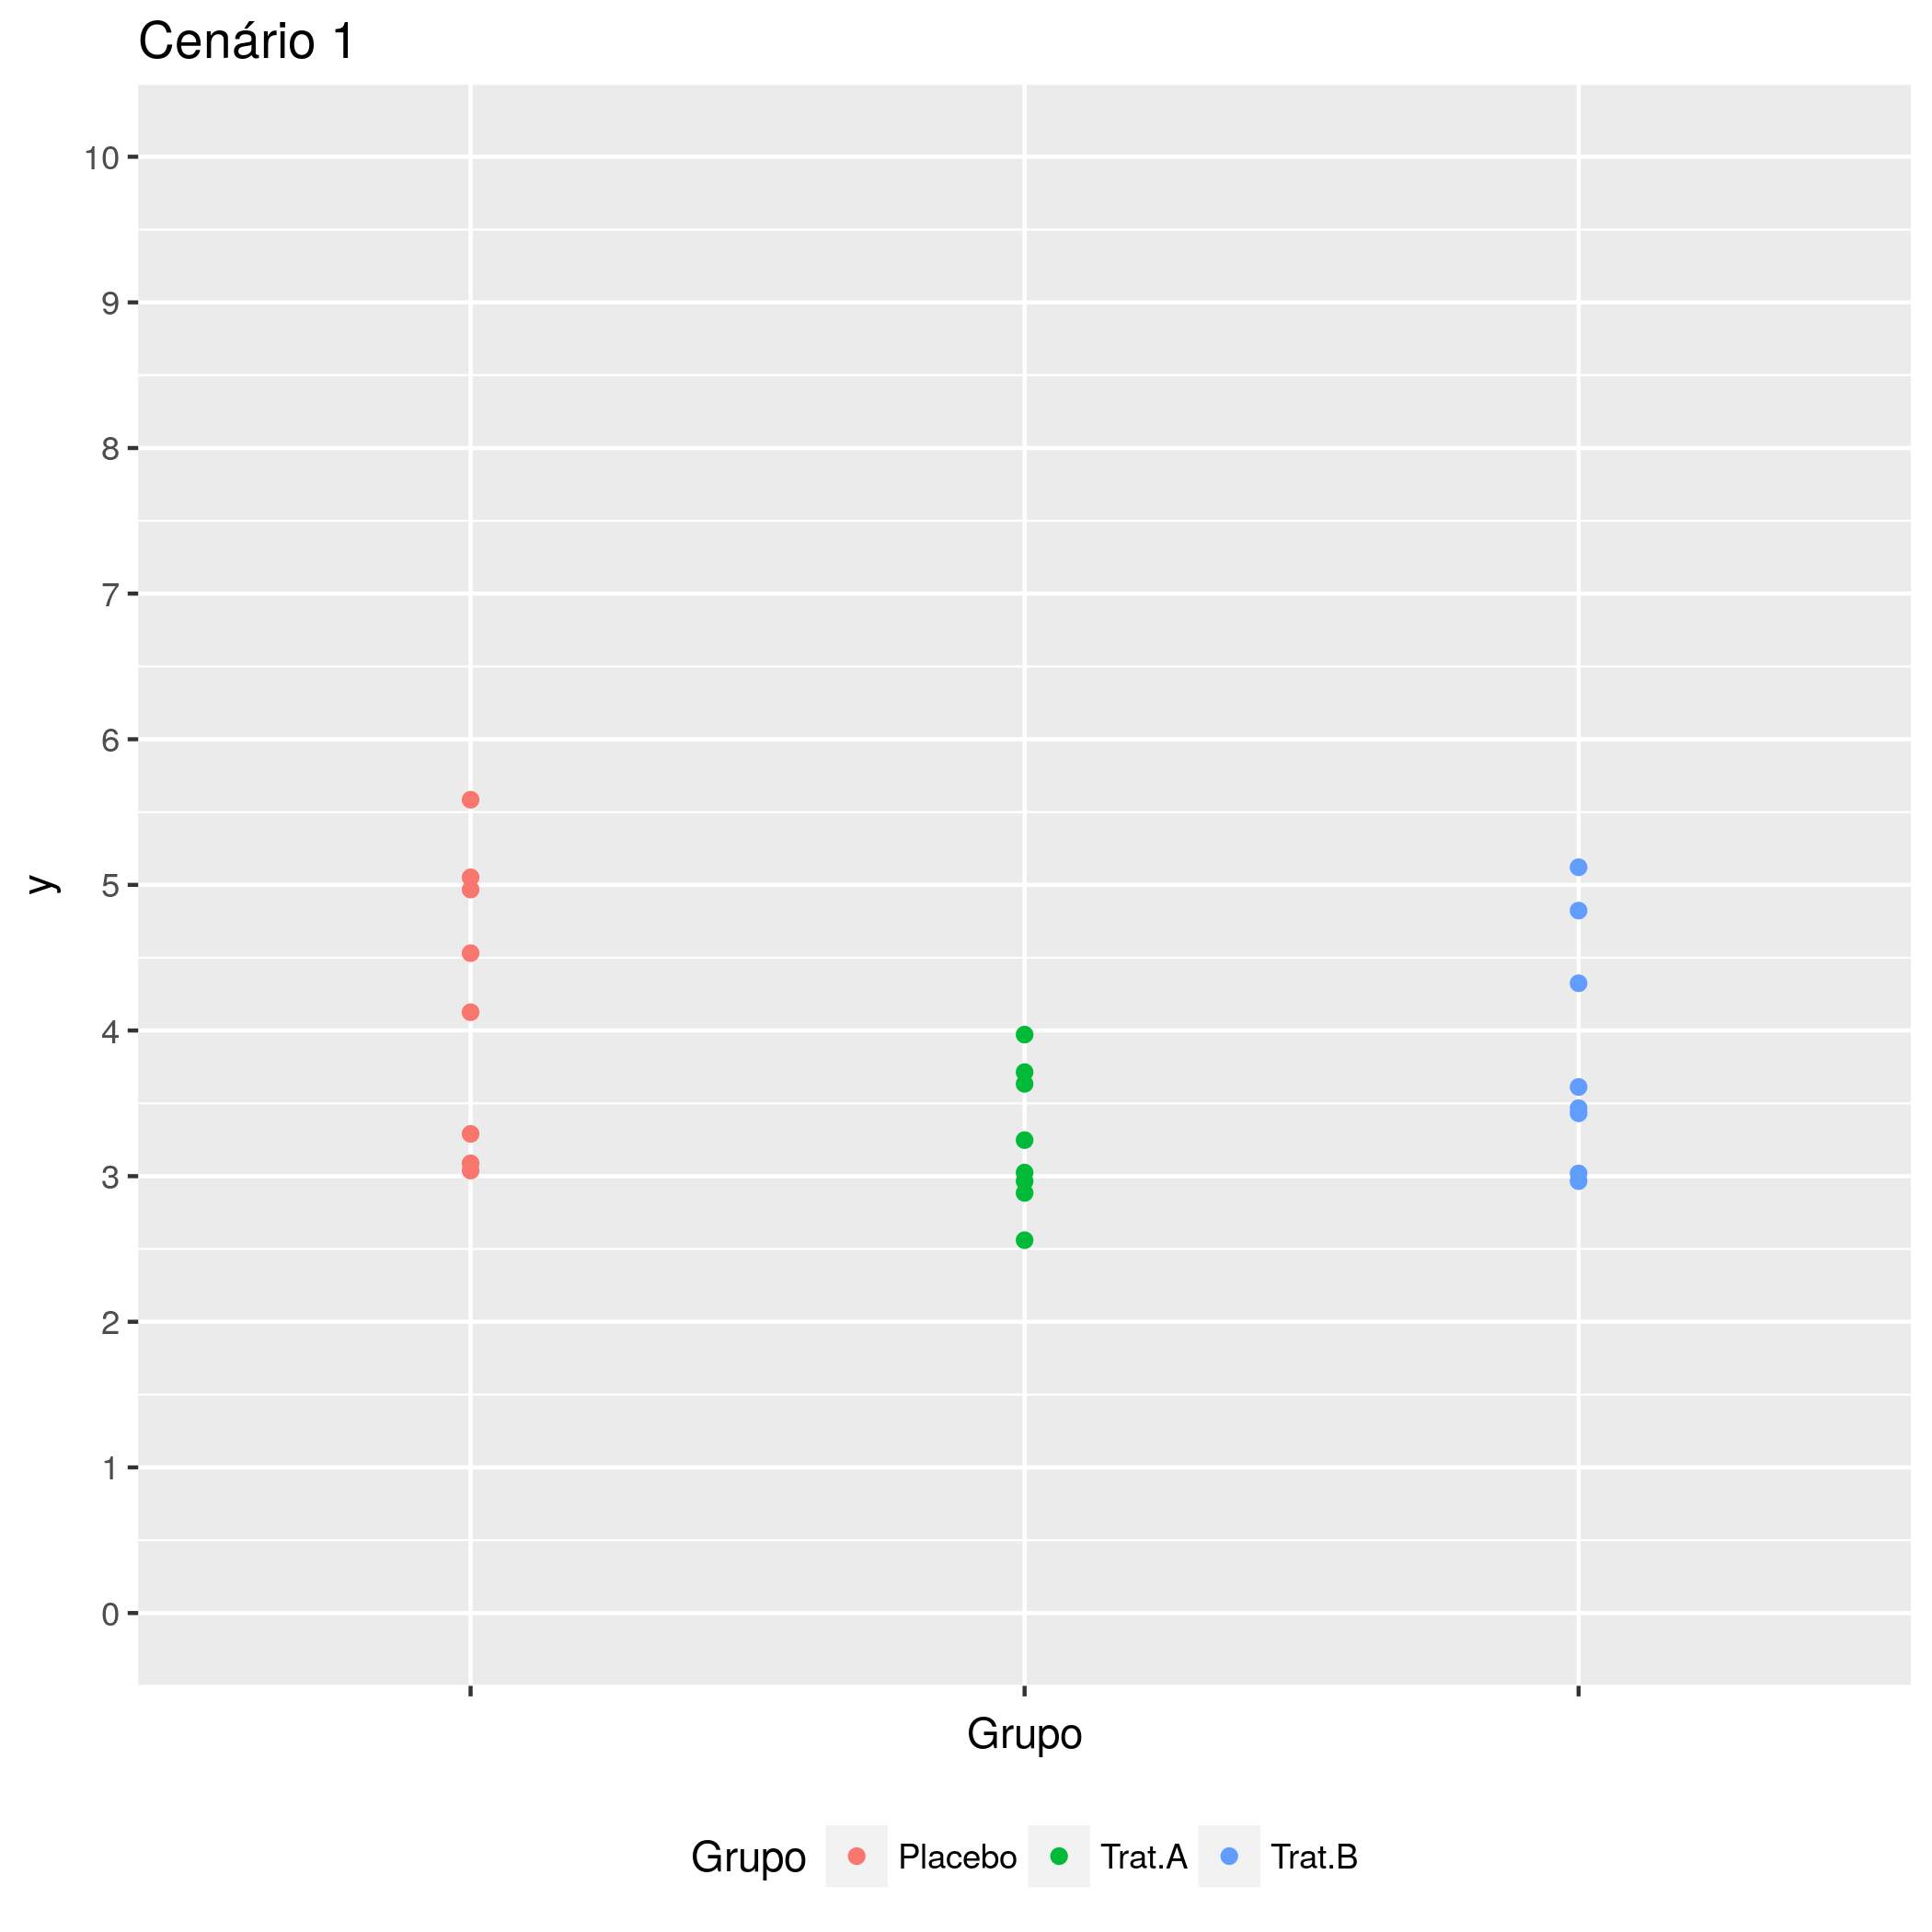
\includegraphics[height=.9\textheight]{Topicos_adv/cenario1}
  \end{center}
\end{frame}

\begin{frame}{Médias: Placebo: 4.210, Tratamento A: 3.250, Tratamento B: 3.845}
  \begin{center}
    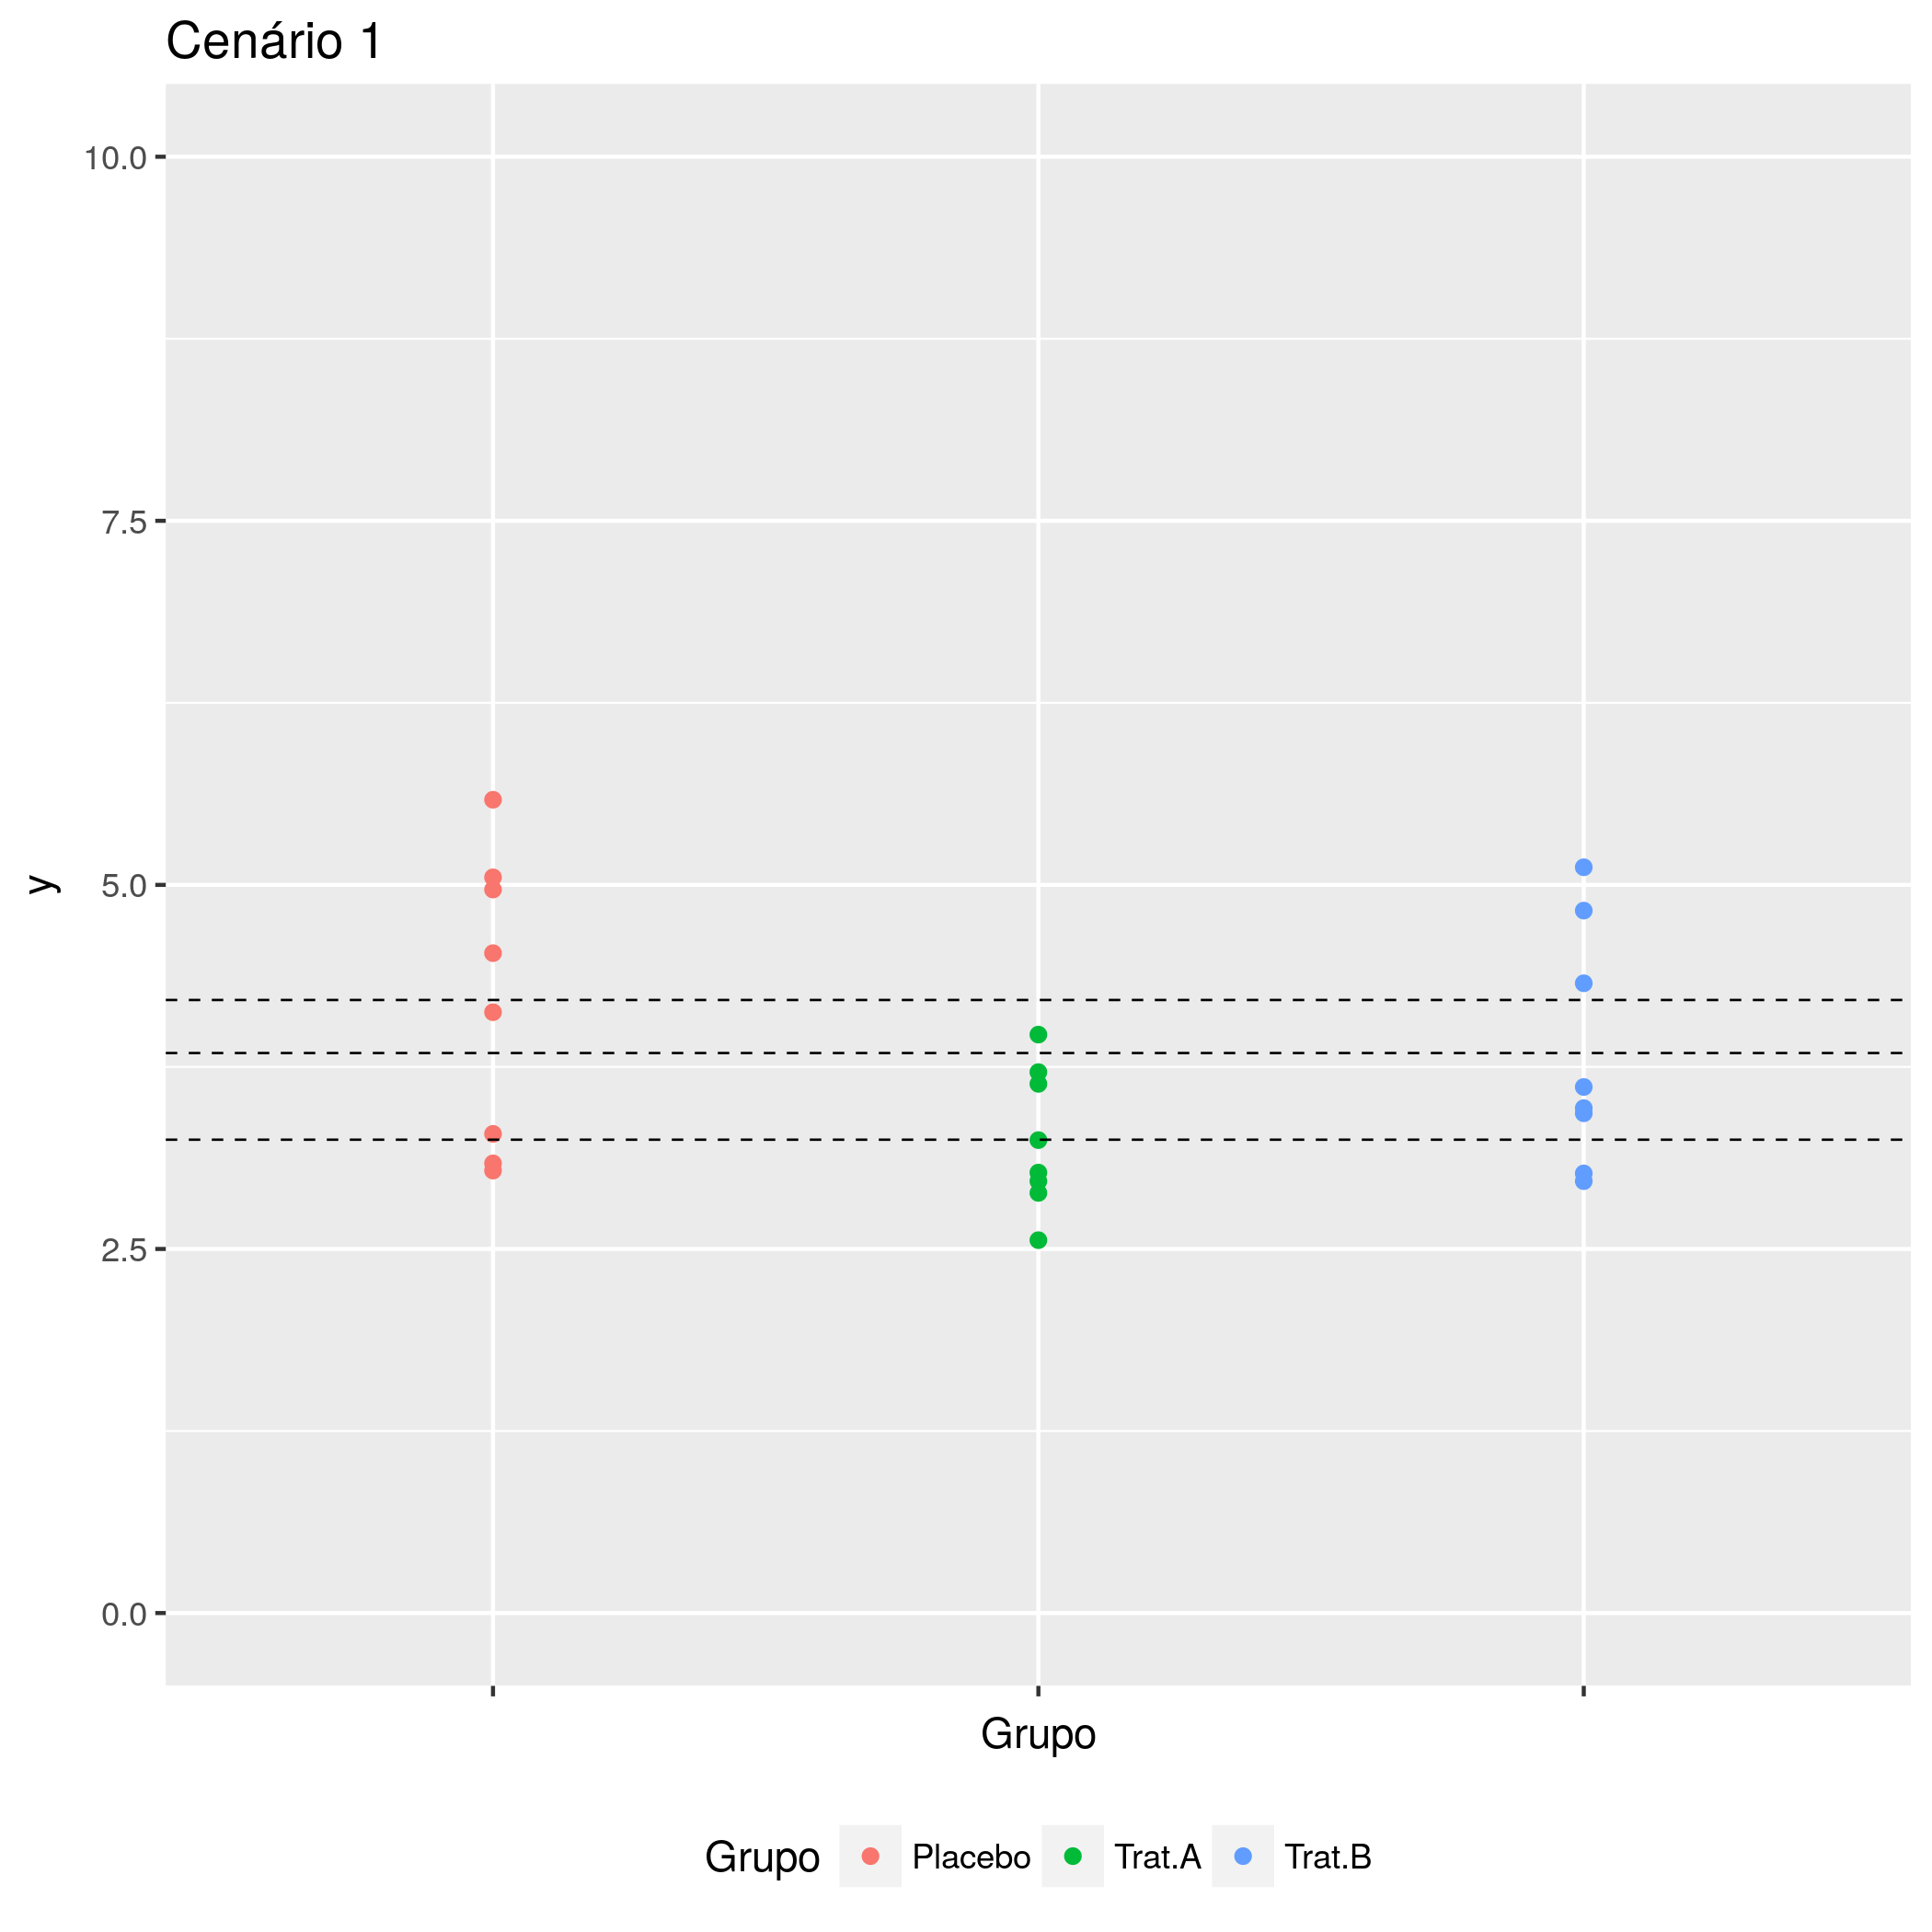
\includegraphics[height=.9\textheight]{Topicos_adv/cenario1_medias}

%    {\tiny Médias: Placebo: 4.210, Tratamento A: 3.250, Tratamento B: 3.845}
  \end{center}
\end{frame}

\begin{frame}{E estes 3 grupos?}
  \begin{center}
    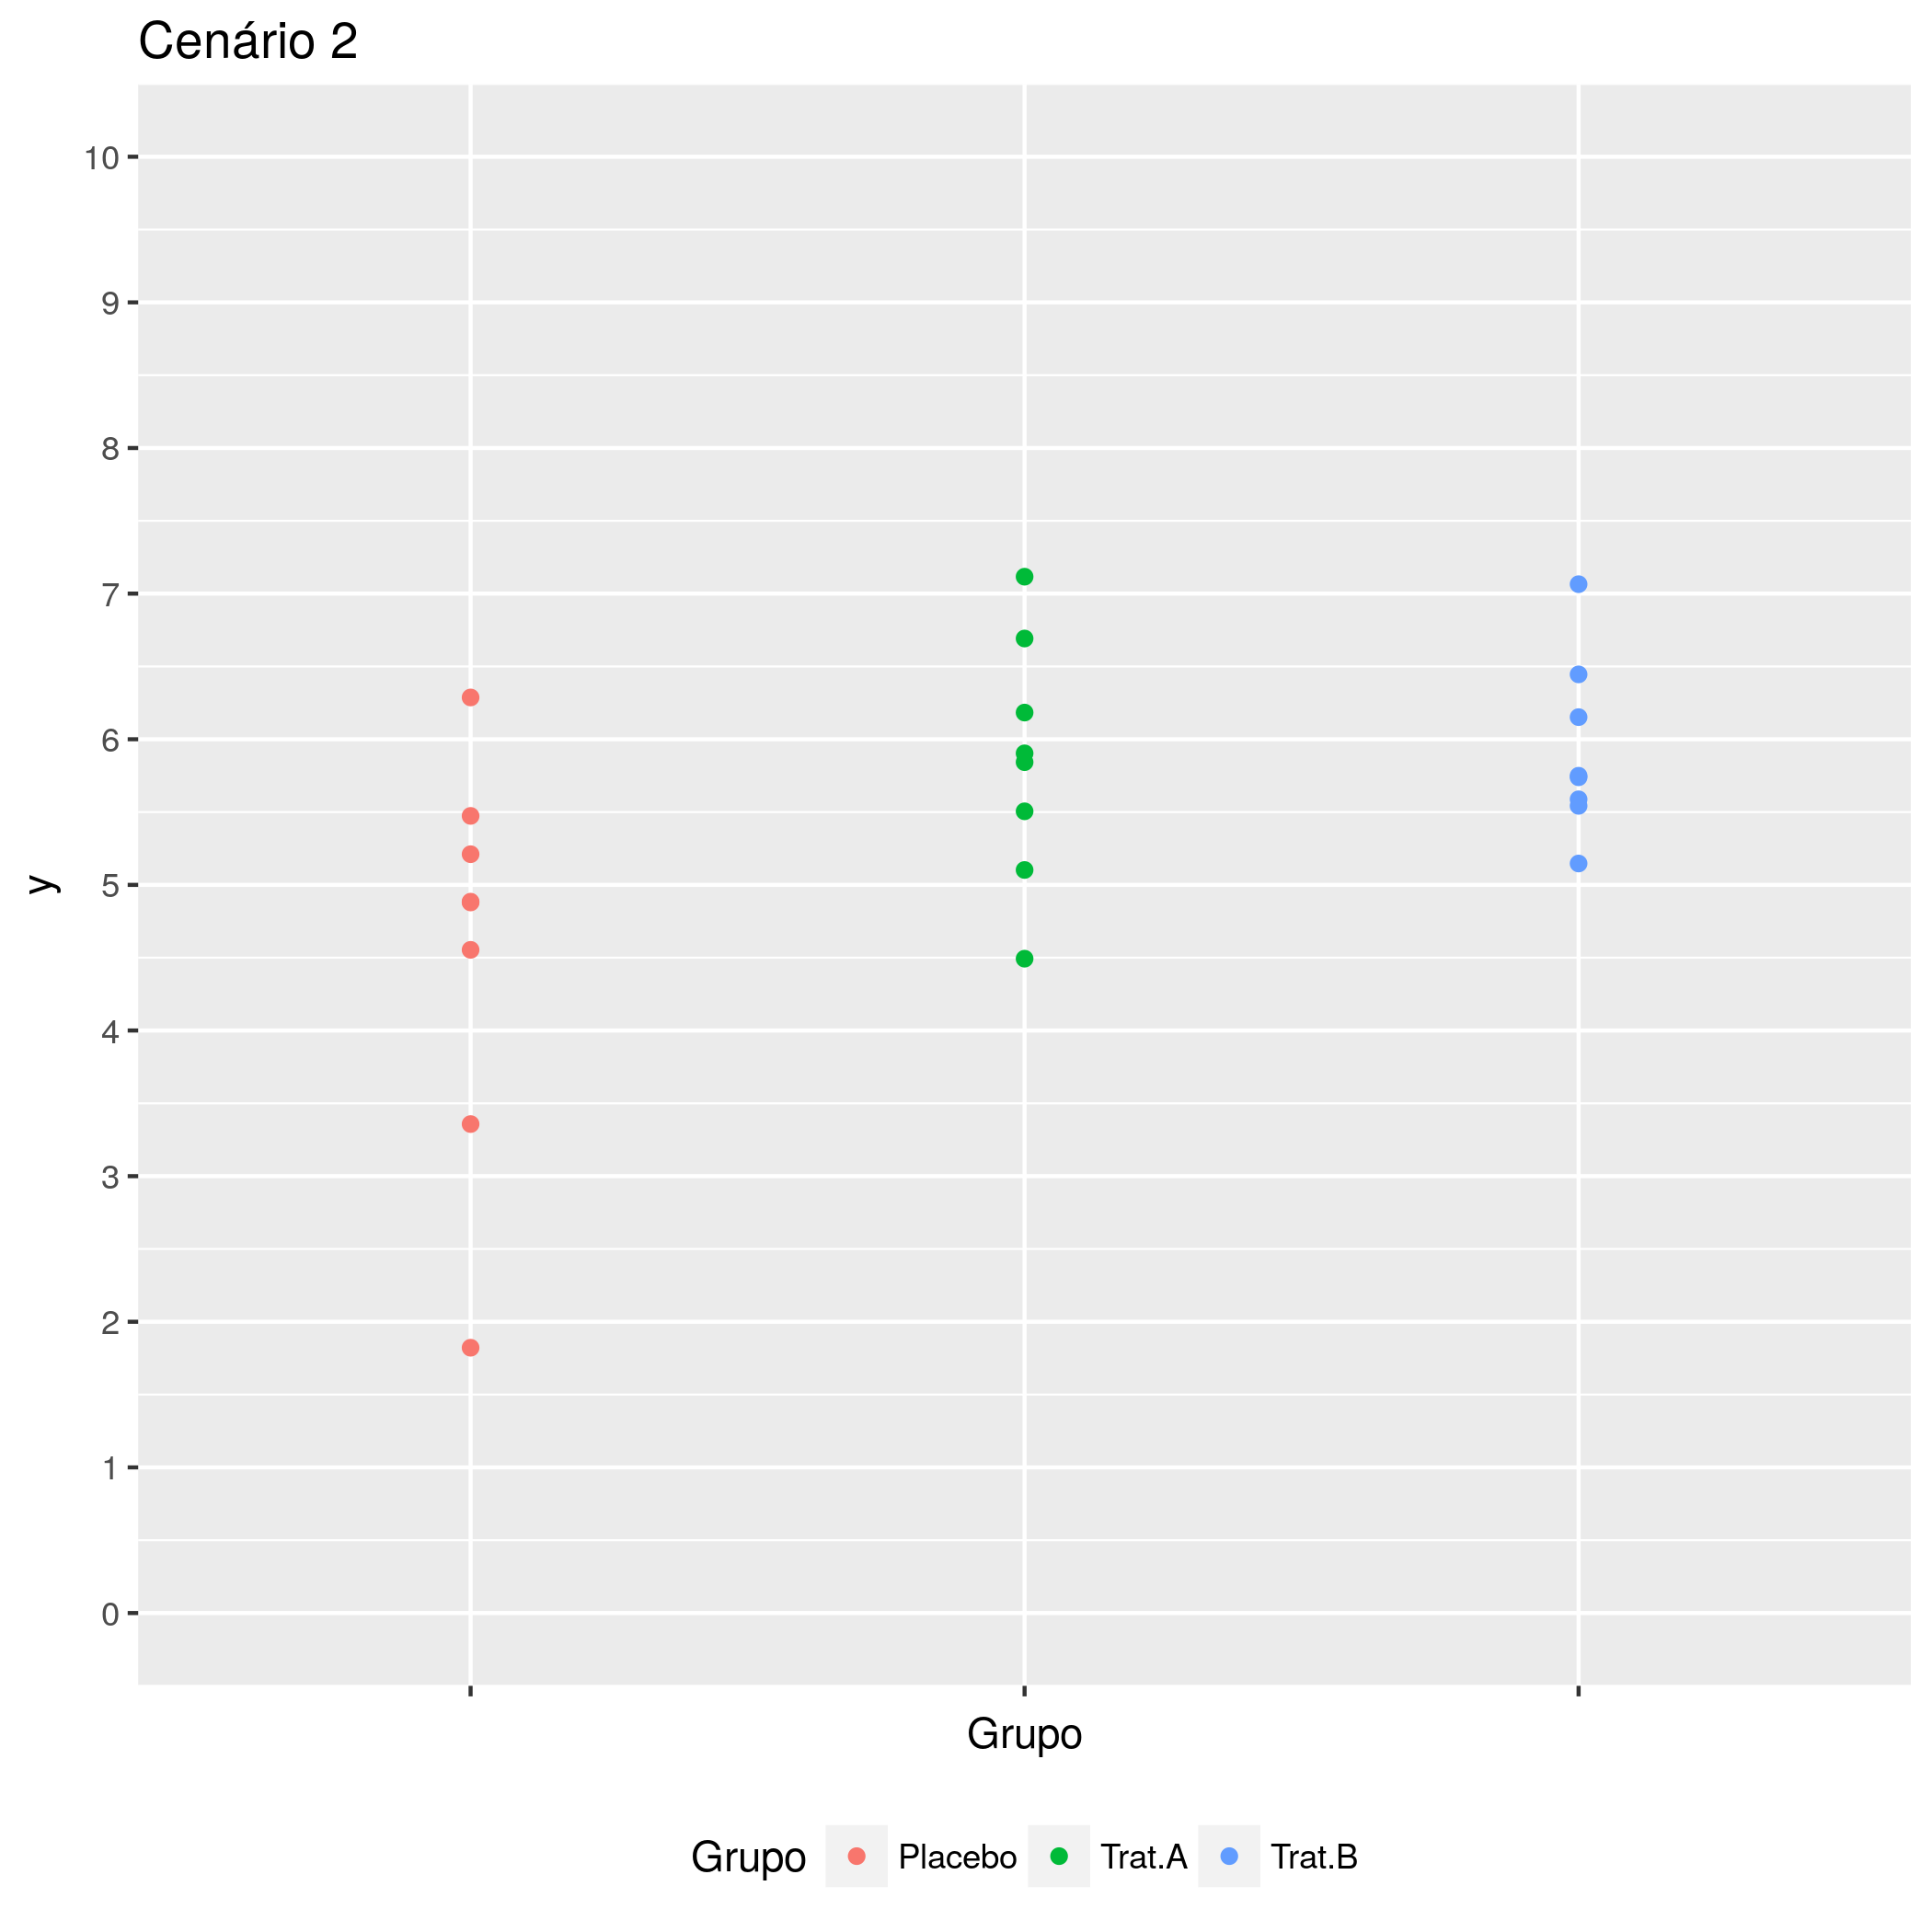
\includegraphics[height=.9\textheight]{Topicos_adv/cenario2}
  \end{center}
\end{frame}

\begin{frame}{Médias: Placebo: 4.559, Tratamento A: 5.855, Tratamento B: 5.928}
  \begin{center}
    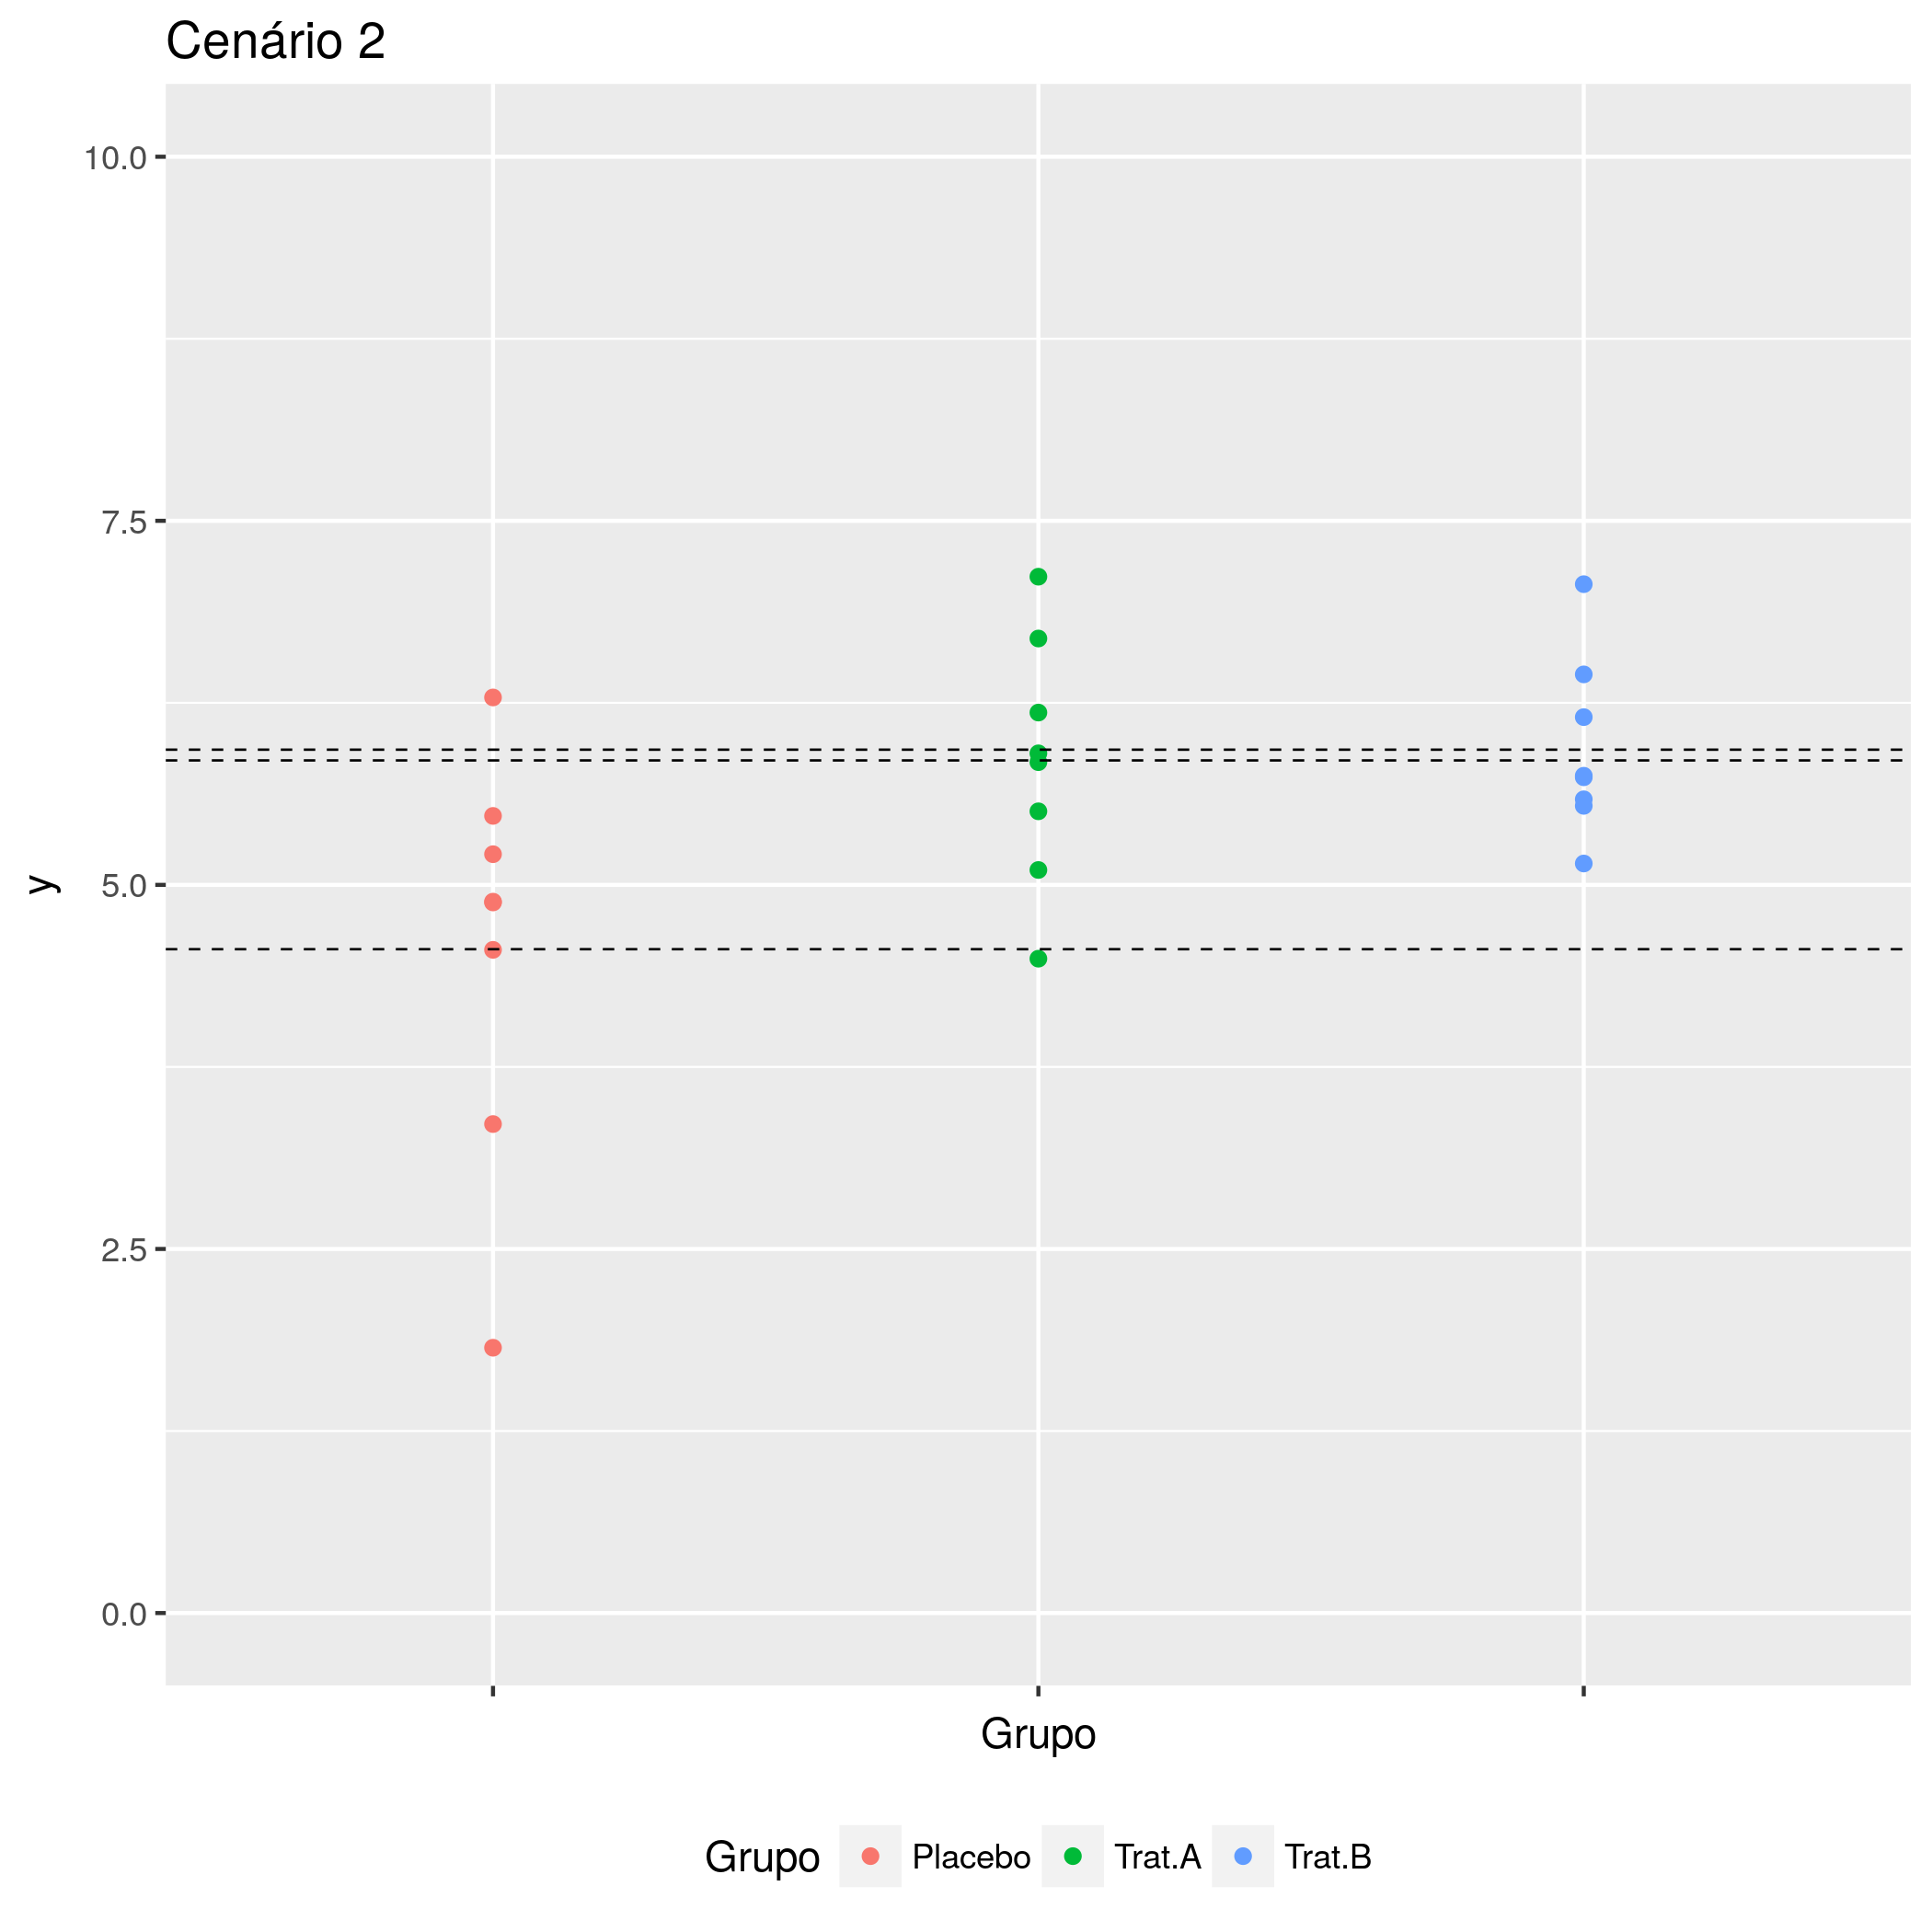
\includegraphics[height=.9\textheight]{Topicos_adv/cenario2_medias}

%    {\tiny Médias: Placebo: 4.559, Tratamento A: 5.855, Tratamento B: 5.928}
  \end{center}
\end{frame}

\begin{frame}{Comparação entre 3 (ou mais) grupos}
  \begin{block}{Abordagem mais simples}
    Uma ideia seria usar o teste t três vezes, comparando os grupos aos pares.

    \bigskip
    Testar se há diferenças significativas, e seus respectivos tamanhos.
  \end{block}

  \begin{exampleblock}{Exemplo}
    \begin{enumerate}
    \item Placebo x Tratamento A
    \item Placebo x Tratamento B
    \item Tratamento A x Tratamento B
    \end{enumerate}
  \end{exampleblock}
\end{frame}

\begin{frame}{Exemplo 1}
  \begin{columns}
    \begin{column}{5cm}
      \begin{exampleblock}{P-valores dos 3 testes t}
        \tiny
        \begin{enumerate}
        \item Placebo x Trat. A $\Rightarrow p=0.02652$
        \item Placebo x Trat. B $\Rightarrow p=0.4331$
        \item Trat. A x Trat. B $\Rightarrow p=0.09686$
        \end{enumerate}
      \end{exampleblock}
      \begin{exampleblock}{Pergunta}
        \small
        Qual é a conclusão correta quanto à comparação destes grupos?
      \end{exampleblock}
    \end{column}
    \begin{column}{5cm}
      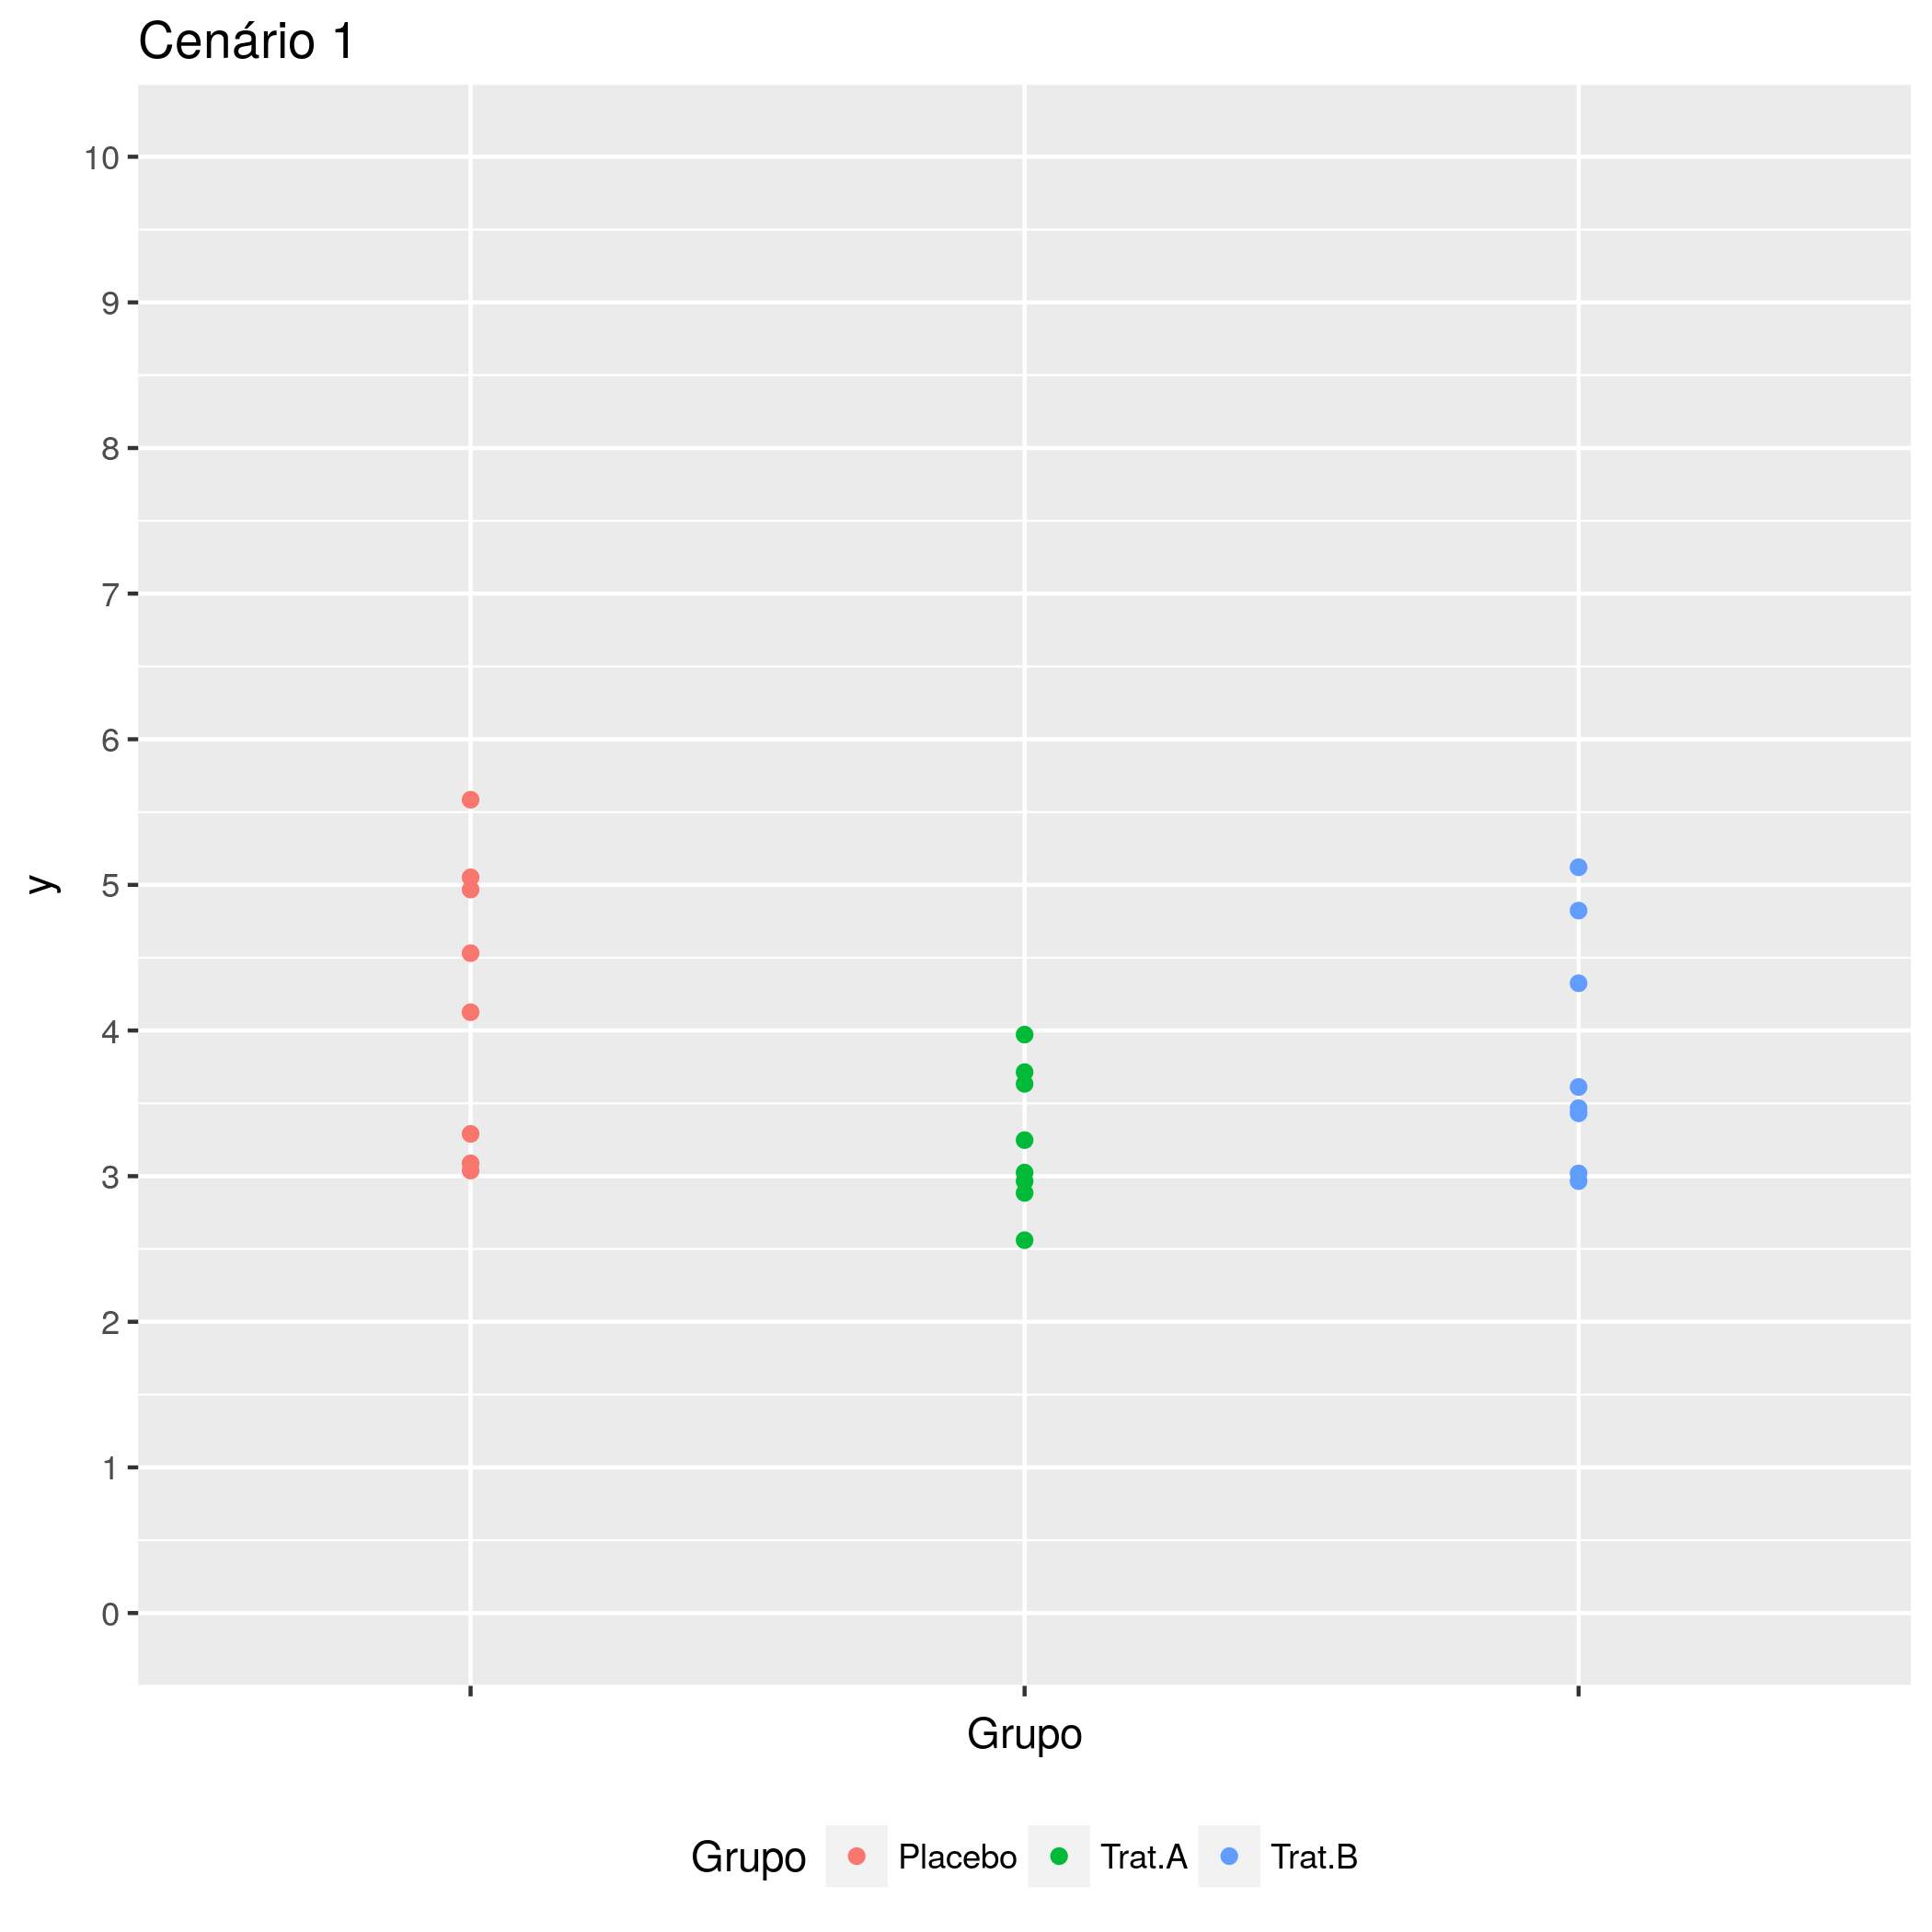
\includegraphics[width=\textwidth]{Topicos_adv/cenario1}
    \end{column}
  \end{columns}
\end{frame}

\begin{frame}{Exemplo 2}
  \begin{columns}
    \begin{column}{5cm}
      \begin{exampleblock}{P-valores dos 3 testes t}
        \tiny
        \begin{enumerate}
        \item Placebo x Trat. A $\Rightarrow p=0.0399$
        \item Placebo x Trat. B $\Rightarrow p=0.02235$
        \item Trat. A x Trat. B $\Rightarrow p=0.8432$
        \end{enumerate}
      \end{exampleblock}
      \begin{exampleblock}{Pergunta}
        \small
        E no segundo cenário?

        Os tratamentos são diferentes do placebo?
        E entre si?
      \end{exampleblock}
    \end{column}
    \begin{column}{5cm}
      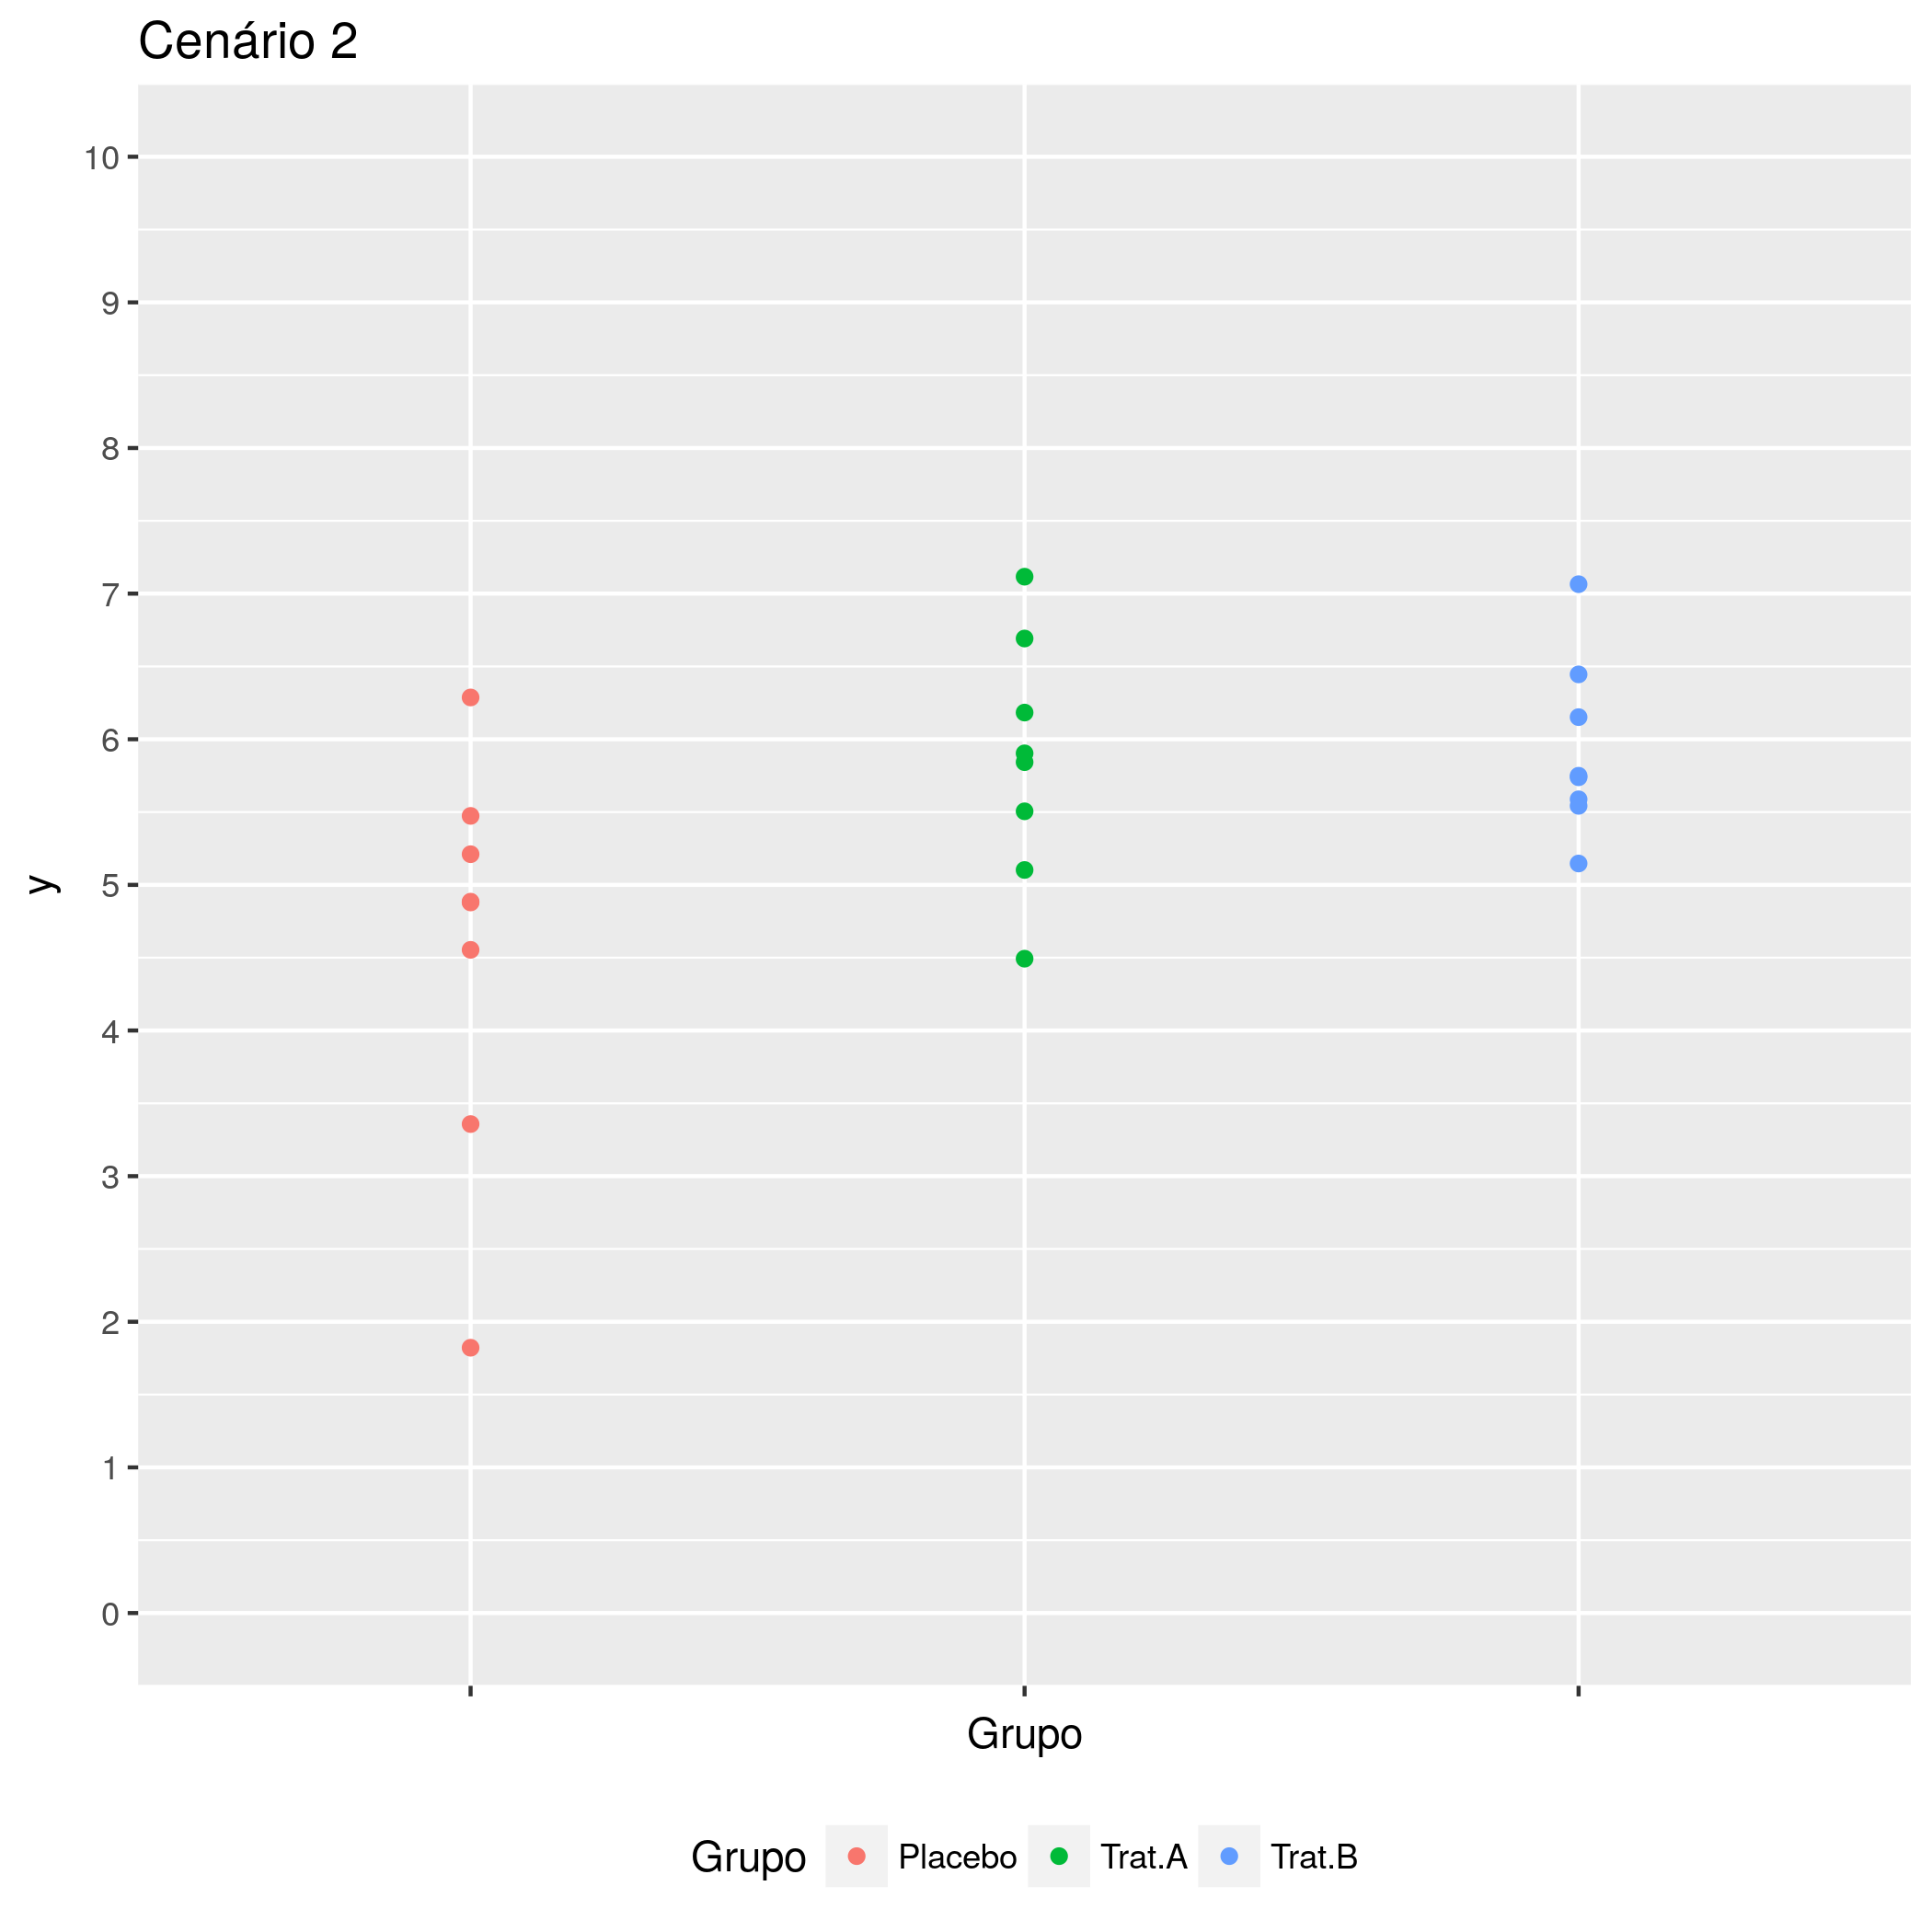
\includegraphics[width=\textwidth]{Topicos_adv/cenario2}
    \end{column}
  \end{columns}
\end{frame}

\begin{frame}{}
  \begin{center}
    Existe um problema oculto aí.
  \end{center}
\end{frame}

\begin{frame}{}
  \begin{center}
    O problema é...
  \end{center}

  % \uncover<2>
  \begin{block}{}<2->
    A conclusão de que no Exemplo 1 os 3 grupos são diferentes está {\bf errada}!
      \end{block}
  \begin{itemize}
  \item<3-> O teste t permite a avaliação de {\bf uma} hipótese
  \item<3-> Testamos simultaneamente várias \footnote{Leia várias vezes o Cap 13!}
  \item<3-> Isto aumenta a chance de cometermos um erro tipo I (falso positivo)
  \item<3-> Múltiplos testes superestimam o p-valor do método
  \end{itemize}
\end{frame}

\begin{frame}{Pensar é obrigatório}
  \begin{itemize}
  \item Os testes estatísticos (e fórmulas) não ``sabem'' o que foi levado em conta no estudo.
  \item {\em Só o pesquisador sabe}
  \item A metodologia da análise precisa levar em conta todo o planejamento do estudo.
  \end{itemize}
\end{frame}

\begin{frame}
  \begin{exampleblock}{Exemplo 13.2}
    5 crianças de uma escola tiveram leucemia, ano passado.

    \begin{itemize}
    \item Isto é uma coincidência?
    \item Esse agrupamento de casos sugere a presença de toxina ou efeito ambiental que causou a doença?

      \bigskip
      {\bf Qual é a probabilidade de se observar 5 casos {\em nesta} escola, em um ano?}
    \end{itemize}
  \end{exampleblock}
\end{frame}

\begin{frame}
  \begin{itemize}
  \item Considerando a incidência de leucemia, isto parece ser um dado extraordinário
  \item Esta é a pergunta errada, {\em após} observar os casos nesta escola.
  \item Se escola não é especial, é preciso considerar outras escolas
  \item Além disso, outras doenças (por ex., asma é um fator?).
  \end{itemize}

\end{frame}
\begin{frame}
  \begin{exampleblock}{Exemplo 13.2}
    5 crianças de uma escola tiveram leucemia, ano passado.

    \begin{itemize}
    \item Isto é uma coincidência?
    \item Esse agrupamento de casos sugere a presença de toxina ou efeito ambiental que causou a doença?

      \bigskip
      {\bf Qual é a probabilidade de se observar 5 casos {\em nesta} escola, em um ano?}
    \end{itemize}
  \end{exampleblock}
  \begin{exampleblock}{Pergunta correta}
    {\bf Qual é a probabilidade de se observar 5 casos {\em em alguma} escola, em um ano?}
  \end{exampleblock}
\end{frame}

\begin{frame}{E agora, José?}
  \begin{block}{}
    Como levar em conta as comparações múltiplas sem ser induzido ao erro, pelo teste t?
  \end{block}
  \bigskip
  \begin{center}
    
\includegraphics[width=.4\textwidth]{Jackie-Chan-WTF}
  \end{center}
\end{frame}

\againframe{requisito}

\section[ANOVA]{Análise de Variância (ANOVA)}

\subsection{ANOVA um fator (One-way ANOVA)}

\begin{frame}[label=exemplo13.5]{Exemplo}
  \begin{exampleblock}{Exemplo 13.5}
    Hetland, et. al (1993) pesquisaram alterações hormonais em mulheres corredoras.
    Mediram o nível de hormônio luteinizante (LH) em três grupos:
    \begin{enumerate}
    \item sedentárias
    \item corredoras recreacionais
    \item corredoras de elite
    \end{enumerate}
  \end{exampleblock}
\end{frame}

\begin{frame}{Exemplo}
  \begin{exampleblock}{Exemplo 13.5}
    \begin{center}
      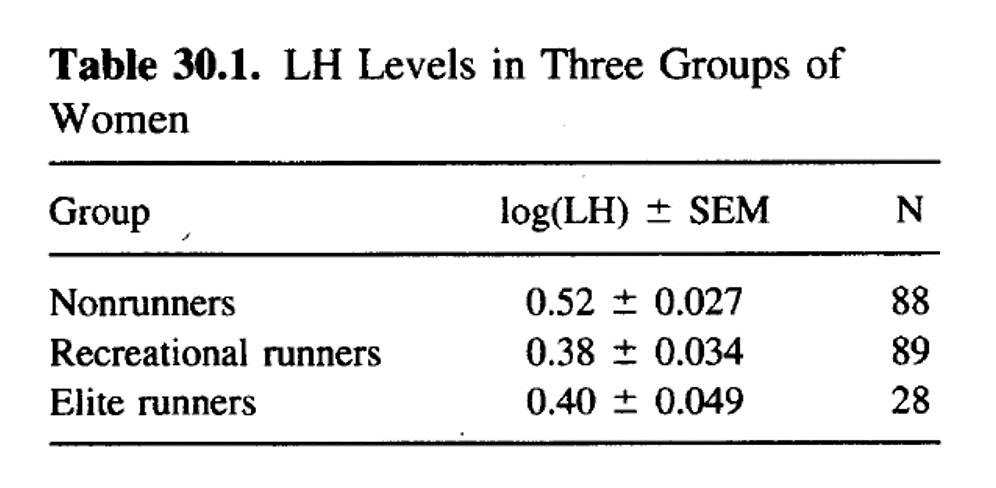
\includegraphics[width=.6\textwidth]{Topicos_adv/exemplo13_5-1}
    \end{center}
  \begin{itemize}
  \item Com estas informações, podemos construir uma tabela ANOVA
  \item $H_0$: todas as médias são iguais
  \end{itemize}
  \end{exampleblock}
\end{frame}

\begin{frame}{Exemplo}
  \begin{exampleblock}{Exemplo 13.5}
    \begin{center}
      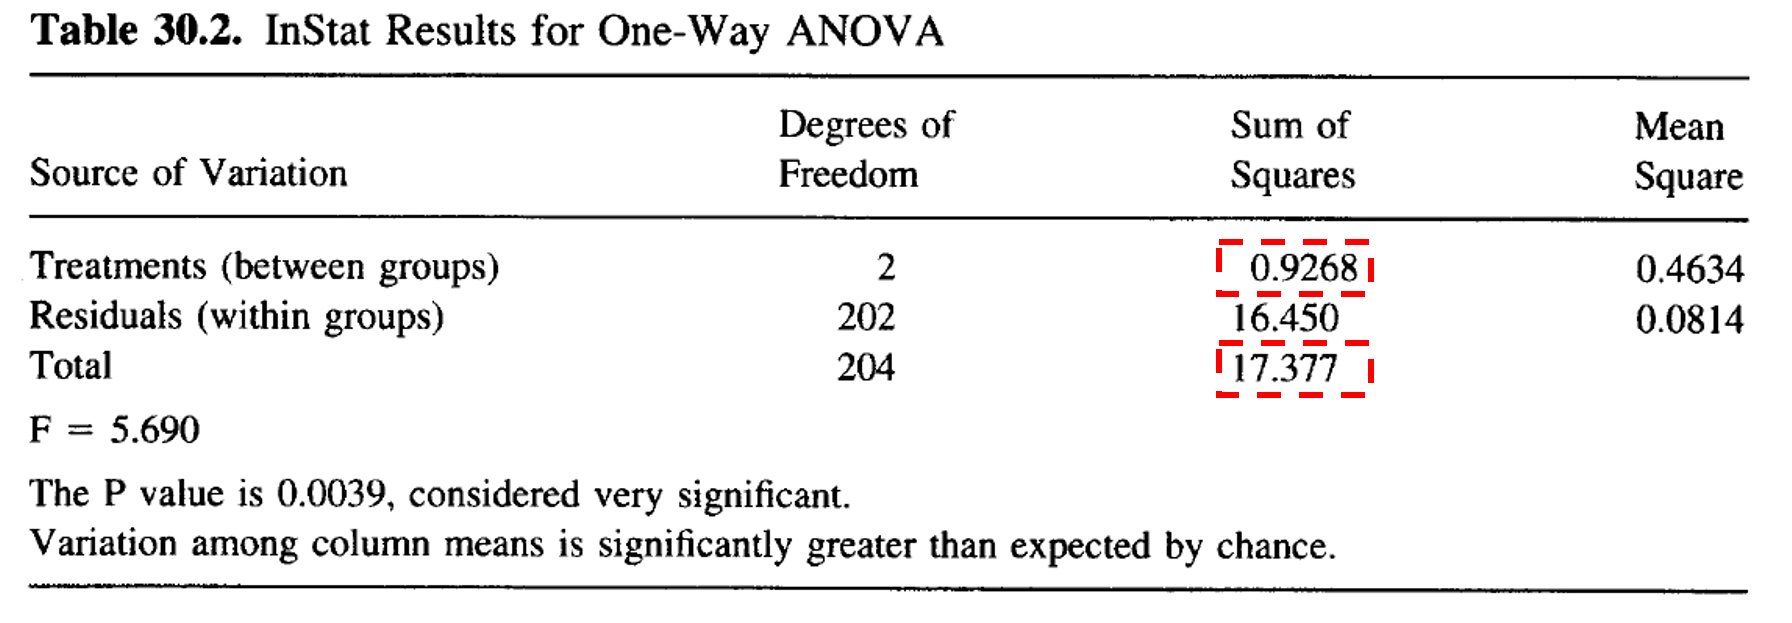
\includegraphics[width=.6\textwidth]{Topicos_adv/exemplo13_5-2}
    \end{center}
  \begin{itemize}
  \item A razão entre as Somas dos Quadrados: $0.93/17.38 = 5.3\%$
  \item $5.3\%$ da variabilidade pode ser explicada pelas diferenças {\em entre os grupos}
  \item (lembra do $r^2?)$
  \end{itemize}
  \end{exampleblock}
\end{frame}

\begin{frame}{One-way ANOVA}
  \begin{itemize}
  \item Este método é chamado one-way (ou 1-way) ANOVA, pois tem um fator categórico
  \item A premissa é que pode-se {\em modelar} a relação entre um desfecho quantitativo e um preditor categórico + um erro aleatório
  \item A variável dependente do exemplo é o LH
  \item A (única) variável independente é o Grupo
  \end{itemize}
\end{frame}

\begin{frame}{A ideia básica}
  \begin{itemize}
  \item Quando os grupos têm médias diferentes, parte da variabilidade total é devido a esta diferença
  \item O resto da variabilidade é devido apenas às variâncias intra-grupos
  % \item Quando as médias são iguais, temos apenas as variâncias intra-grupos e inter-grupos.
  \item A ANOVA tenta {\em desembaraçar} esta decomposição, assumindo a hipótese nula.
  \end{itemize}
\end{frame}

\begin{frame}{A ideia básica}
  \begin{itemize}
  \item O nome {\em Análise de Variância} vem do critério usado para comparar as médias
  \item O teste de hipótese é baseado na comparação entre as variâncias intra- e inter grupos
  \end{itemize}
\end{frame}

% > summary(anova1)
%             Df Sum Sq Mean Sq F value Pr(>F)  
% Grupo        2  3.753  1.8763   3.025 0.0701 .
% Residuals   21 13.026  0.6203                 
% ---
% Signif. codes:  0 ‘***’ 0.001 ‘**’ 0.01 ‘*’ 0.05 ‘.’ 0.1 ‘ ’ 1
% > summary(anova12)
%             Df Sum Sq Mean Sq F value Pr(>F)  
% Grupo        2  3.753  1.8763   3.064 0.0691 .
% Genero       1  0.779  0.7792   1.272 0.2727  
% Residuals   20 12.247  0.6123                 
% ---
% Signif. codes:  0 ‘***’ 0.001 ‘**’ 0.01 ‘*’ 0.05 ‘.’ 0.1 ‘ ’ 1
% > summary(anova2)
%             Df Sum Sq Mean Sq F value Pr(>F)  
% Grupo        2  9.499   4.749   4.775 0.0195 *
% Residuals   21 20.889   0.995                 
% ---
% Signif. codes:  0 ‘***’ 0.001 ‘**’ 0.01 ‘*’ 0.05 ‘.’ 0.1 ‘ ’ 1
% > summary(anova22)
%             Df Sum Sq Mean Sq F value Pr(>F)  
% Grupo        2  9.499   4.749   4.548 0.0236 *
% Genero       1  0.002   0.002   0.002 0.9690  
% Residuals   20 20.887   1.044                 
% ---
% Signif. codes:  0 ‘***’ 0.001 ‘**’ 0.01 ‘*’ 0.05 ‘.’ 0.1 ‘ ’ 1

% > TukeyHSD(anova1)
%   Tukey multiple comparisons of means
%     95% family-wise confidence level

% Fit: aov(formula = y ~ Grupo, data = cenario1.long)

% $Grupo
%                      diff       lwr        upr     p adj
% Trat.A-Placebo -0.9593453 -1.951928 0.03323713 0.0593745
% Trat.B-Placebo -0.3641649 -1.356747 0.62841756 0.6310533
% Trat.B-Trat.A   0.5951804 -0.397402 1.58776285 0.3059643

% > TukeyHSD(anova12)
%   Tukey multiple comparisons of means
%     95% family-wise confidence level

% Fit: aov(formula = y ~ Grupo + Genero, data = cenario1.long)

% $Grupo
%                      diff        lwr        upr     p adj
% Trat.A-Placebo -0.9593453 -1.9492340 0.03054344 0.0585261
% Trat.B-Placebo -0.3641649 -1.3540536 0.62572388 0.6277051
% Trat.B-Trat.A   0.5951804 -0.3947083 1.58506917 0.3025618

% $Genero
%          diff       lwr      upr     p adj
% M-F 0.4161096 -0.353374 1.185593 0.2726642

% > TukeyHSD(anova2)
%   Tukey multiple comparisons of means
%     95% family-wise confidence level

% Fit: aov(formula = y ~ Grupo, data = cenario2.long)

% $Grupo
%                      diff        lwr      upr     p adj
% Trat.A-Placebo 1.29615978  0.0392117 2.553108 0.0424949
% Trat.B-Placebo 1.36988994  0.1129419 2.626838 0.0311078
% Trat.B-Trat.A  0.07373016 -1.1832179 1.330678 0.9880276

% > TukeyHSD(anova22)
%   Tukey multiple comparisons of means
%     95% family-wise confidence level

% Fit: aov(formula = y ~ Grupo + Genero, data = cenario2.long)

% $Grupo
%                      diff          lwr      upr     p adj
% Trat.A-Placebo 1.29615978  0.003412143 2.588907 0.0493258
% Trat.B-Placebo 1.36988994  0.077142303 2.662638 0.0366413
% Trat.B-Trat.A  0.07373016 -1.219017478 1.366478 0.9885936

% $Genero
%            diff        lwr       upr     p adj
% M-F -0.01696485 -0.9157828 0.8818531 0.9689844

% > anova1.p.bonf

% 	Pairwise comparisons using t tests with pooled SD 

% data:  y and Grupo 

%        Placebo Trat.A
% Trat.A 0.072   -     
% Trat.B 1.000   0.437 

% P value adjustment method: bonferroni 
% > anova2.p.bonf

% 	Pairwise comparisons using t tests with pooled SD 

% data:  y and Grupo 

%        Placebo Trat.A
% Trat.A 0.050   -     
% Trat.B 0.036   1.000 

% P value adjustment method: bonferroni 

% > summary(aov(y ~ Grupo + Genero, cenario2.long))
%             Df Sum Sq Mean Sq F value Pr(>F)  
% Grupo        2  9.499   4.749   4.548 0.0236 *
% Genero       1  0.002   0.002   0.002 0.9690  
% Residuals   20 20.887   1.044                 
% ---
% Signif. codes:  0 ‘***’ 0.001 ‘**’ 0.01 ‘*’ 0.05 ‘.’ 0.1 ‘ ’ 1
% > summary(aov(y ~ Grupo * Genero, cenario2.long))
%              Df Sum Sq Mean Sq F value Pr(>F)  
% Grupo         2  9.499   4.749   4.707 0.0227 *
% Genero        1  0.002   0.002   0.002 0.9685  
% Grupo:Genero  2  2.725   1.362   1.350 0.2842  
% Residuals    18 18.163   1.009                 
% ---
% Signif. codes:  0 ‘***’ 0.001 ‘**’ 0.01 ‘*’ 0.05 ‘.’ 0.1 ‘ ’ 1

% > TukeyHSD(aov(y ~ Grupo * Genero, cenario2.long))
%   Tukey multiple comparisons of means
%     95% family-wise confidence level

% Fit: aov(formula = y ~ Grupo * Genero, data = cenario2.long)

% $Grupo
%                     diff        lwr      upr     p adj
% Trat.A-Placebo 1.5514853  0.2712011 2.831770 0.0164455
% Trat.B-Placebo 2.1703237  0.8900395 3.450608 0.0011265
% Trat.B-Trat.A  0.6188384 -0.6614458 1.899123 0.4494538

% $Genero
%          diff         lwr      upr     p adj
% M-F 0.8071626 -0.08158125 1.695906 0.0724633

% $`Grupo:Genero`
%                           diff        lwr      upr     p adj
% Trat.A:F-Placebo:F   2.1160544 -0.4873461 4.719455 0.1523427
% Trat.B:F-Placebo:F   1.5879521 -1.0154484 4.191353 0.4122593
% Placebo:M-Placebo:F  0.7976679 -1.5308843 3.126220 0.8795976
% Trat.A:M-Placebo:F   2.0104118 -0.3181404 4.338964 0.1143524
% Trat.B:M-Placebo:F   3.3174146  0.9888624 5.645967 0.0030192
% Trat.B:F-Trat.A:F   -0.5281023 -3.1315028 2.075298 0.9857698
% Placebo:M-Trat.A:F  -1.3183865 -3.6469387 1.010166 0.4902167
% Trat.A:M-Trat.A:F   -0.1056426 -2.4341948 2.222910 0.9999896
% Trat.B:M-Trat.A:F    1.2013602 -1.1271920 3.529912 0.5849474
% Placebo:M-Trat.B:F  -0.7902842 -3.1188364 1.538268 0.8835616
% Trat.A:M-Trat.B:F    0.4224597 -1.9060925 2.751012 0.9913898
% Trat.B:M-Trat.B:F    1.7294625 -0.5990897 4.058015 0.2216761
% Trat.A:M-Placebo:M   1.2127439 -0.8038415 3.229329 0.4270508
% Trat.B:M-Placebo:M   2.5197467  0.5031614 4.536332 0.0098078
% Trat.B:M-Trat.A:M    1.3070028 -0.7095825 3.323588 0.3496917

% \begin{frame}{3 grupos - cenário 1}
%   \begin{center}
%     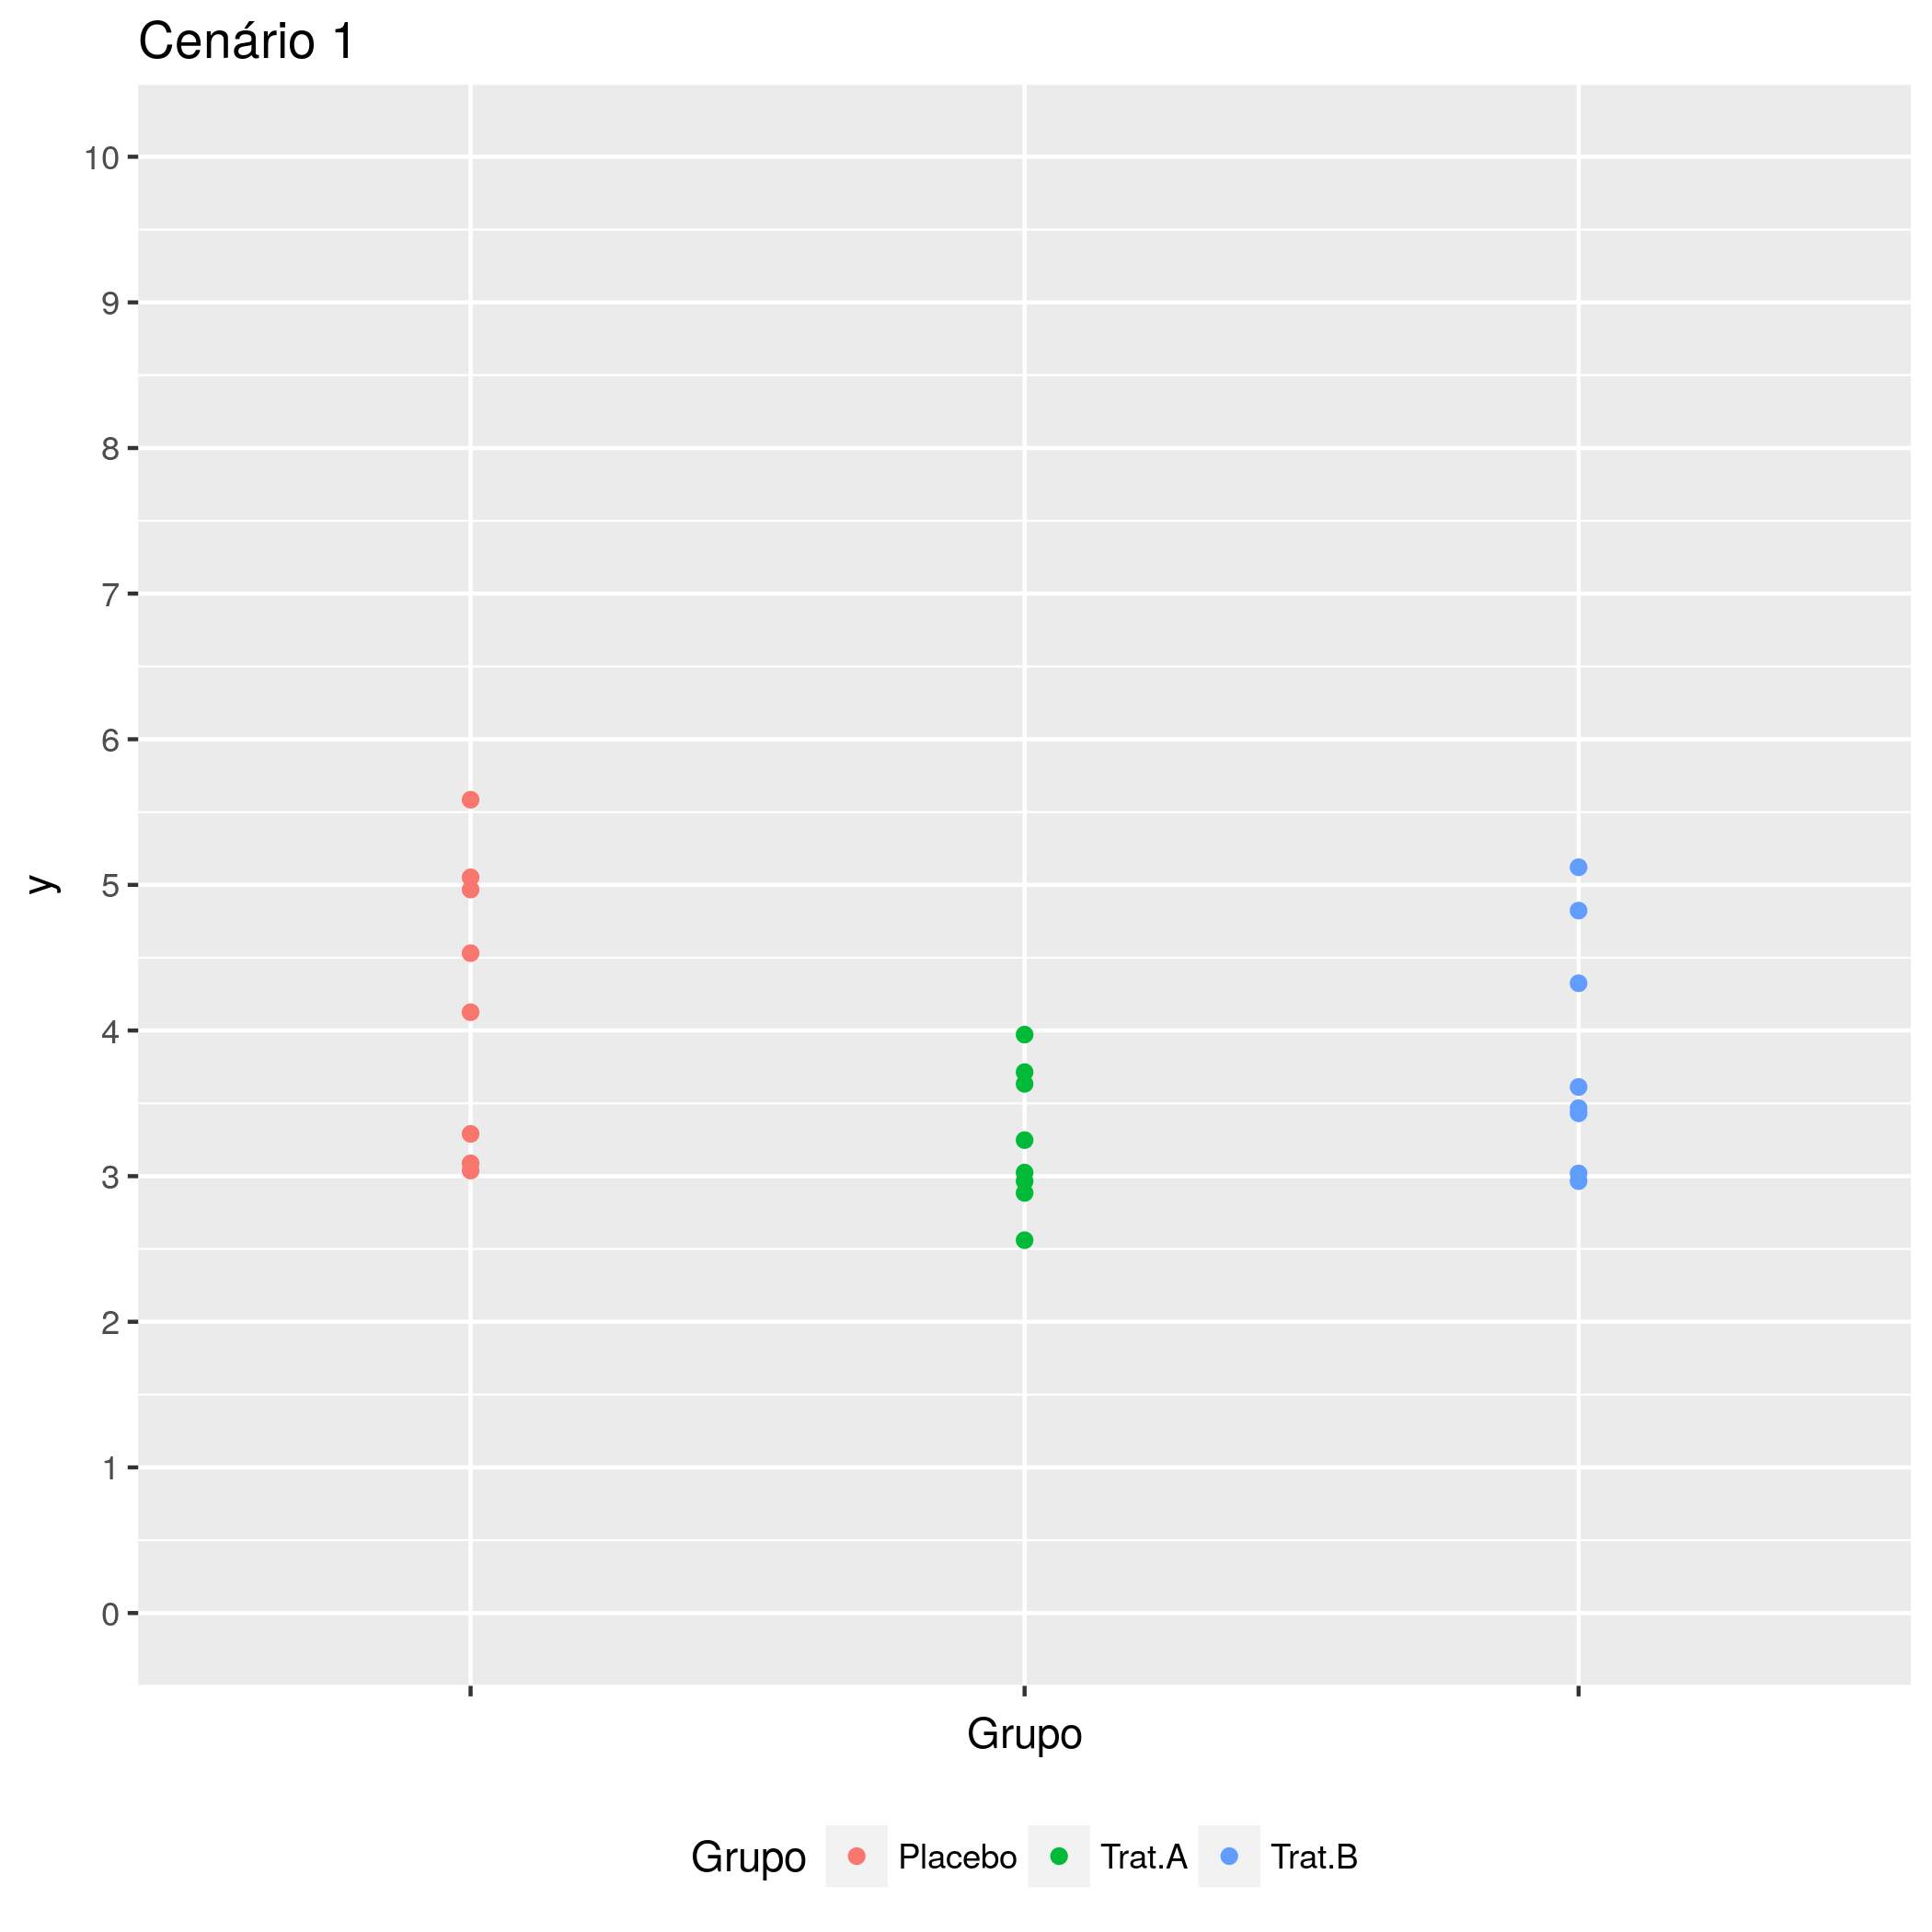
\includegraphics[height=.9\textheight]{Topicos_adv/cenario1}
%   \end{center}
% \end{frame}

% \begin{frame}{Médias: Placebo: 4.210, Tratamento A: 3.250, Tratamento B: 3.845}
%   \begin{center}
%     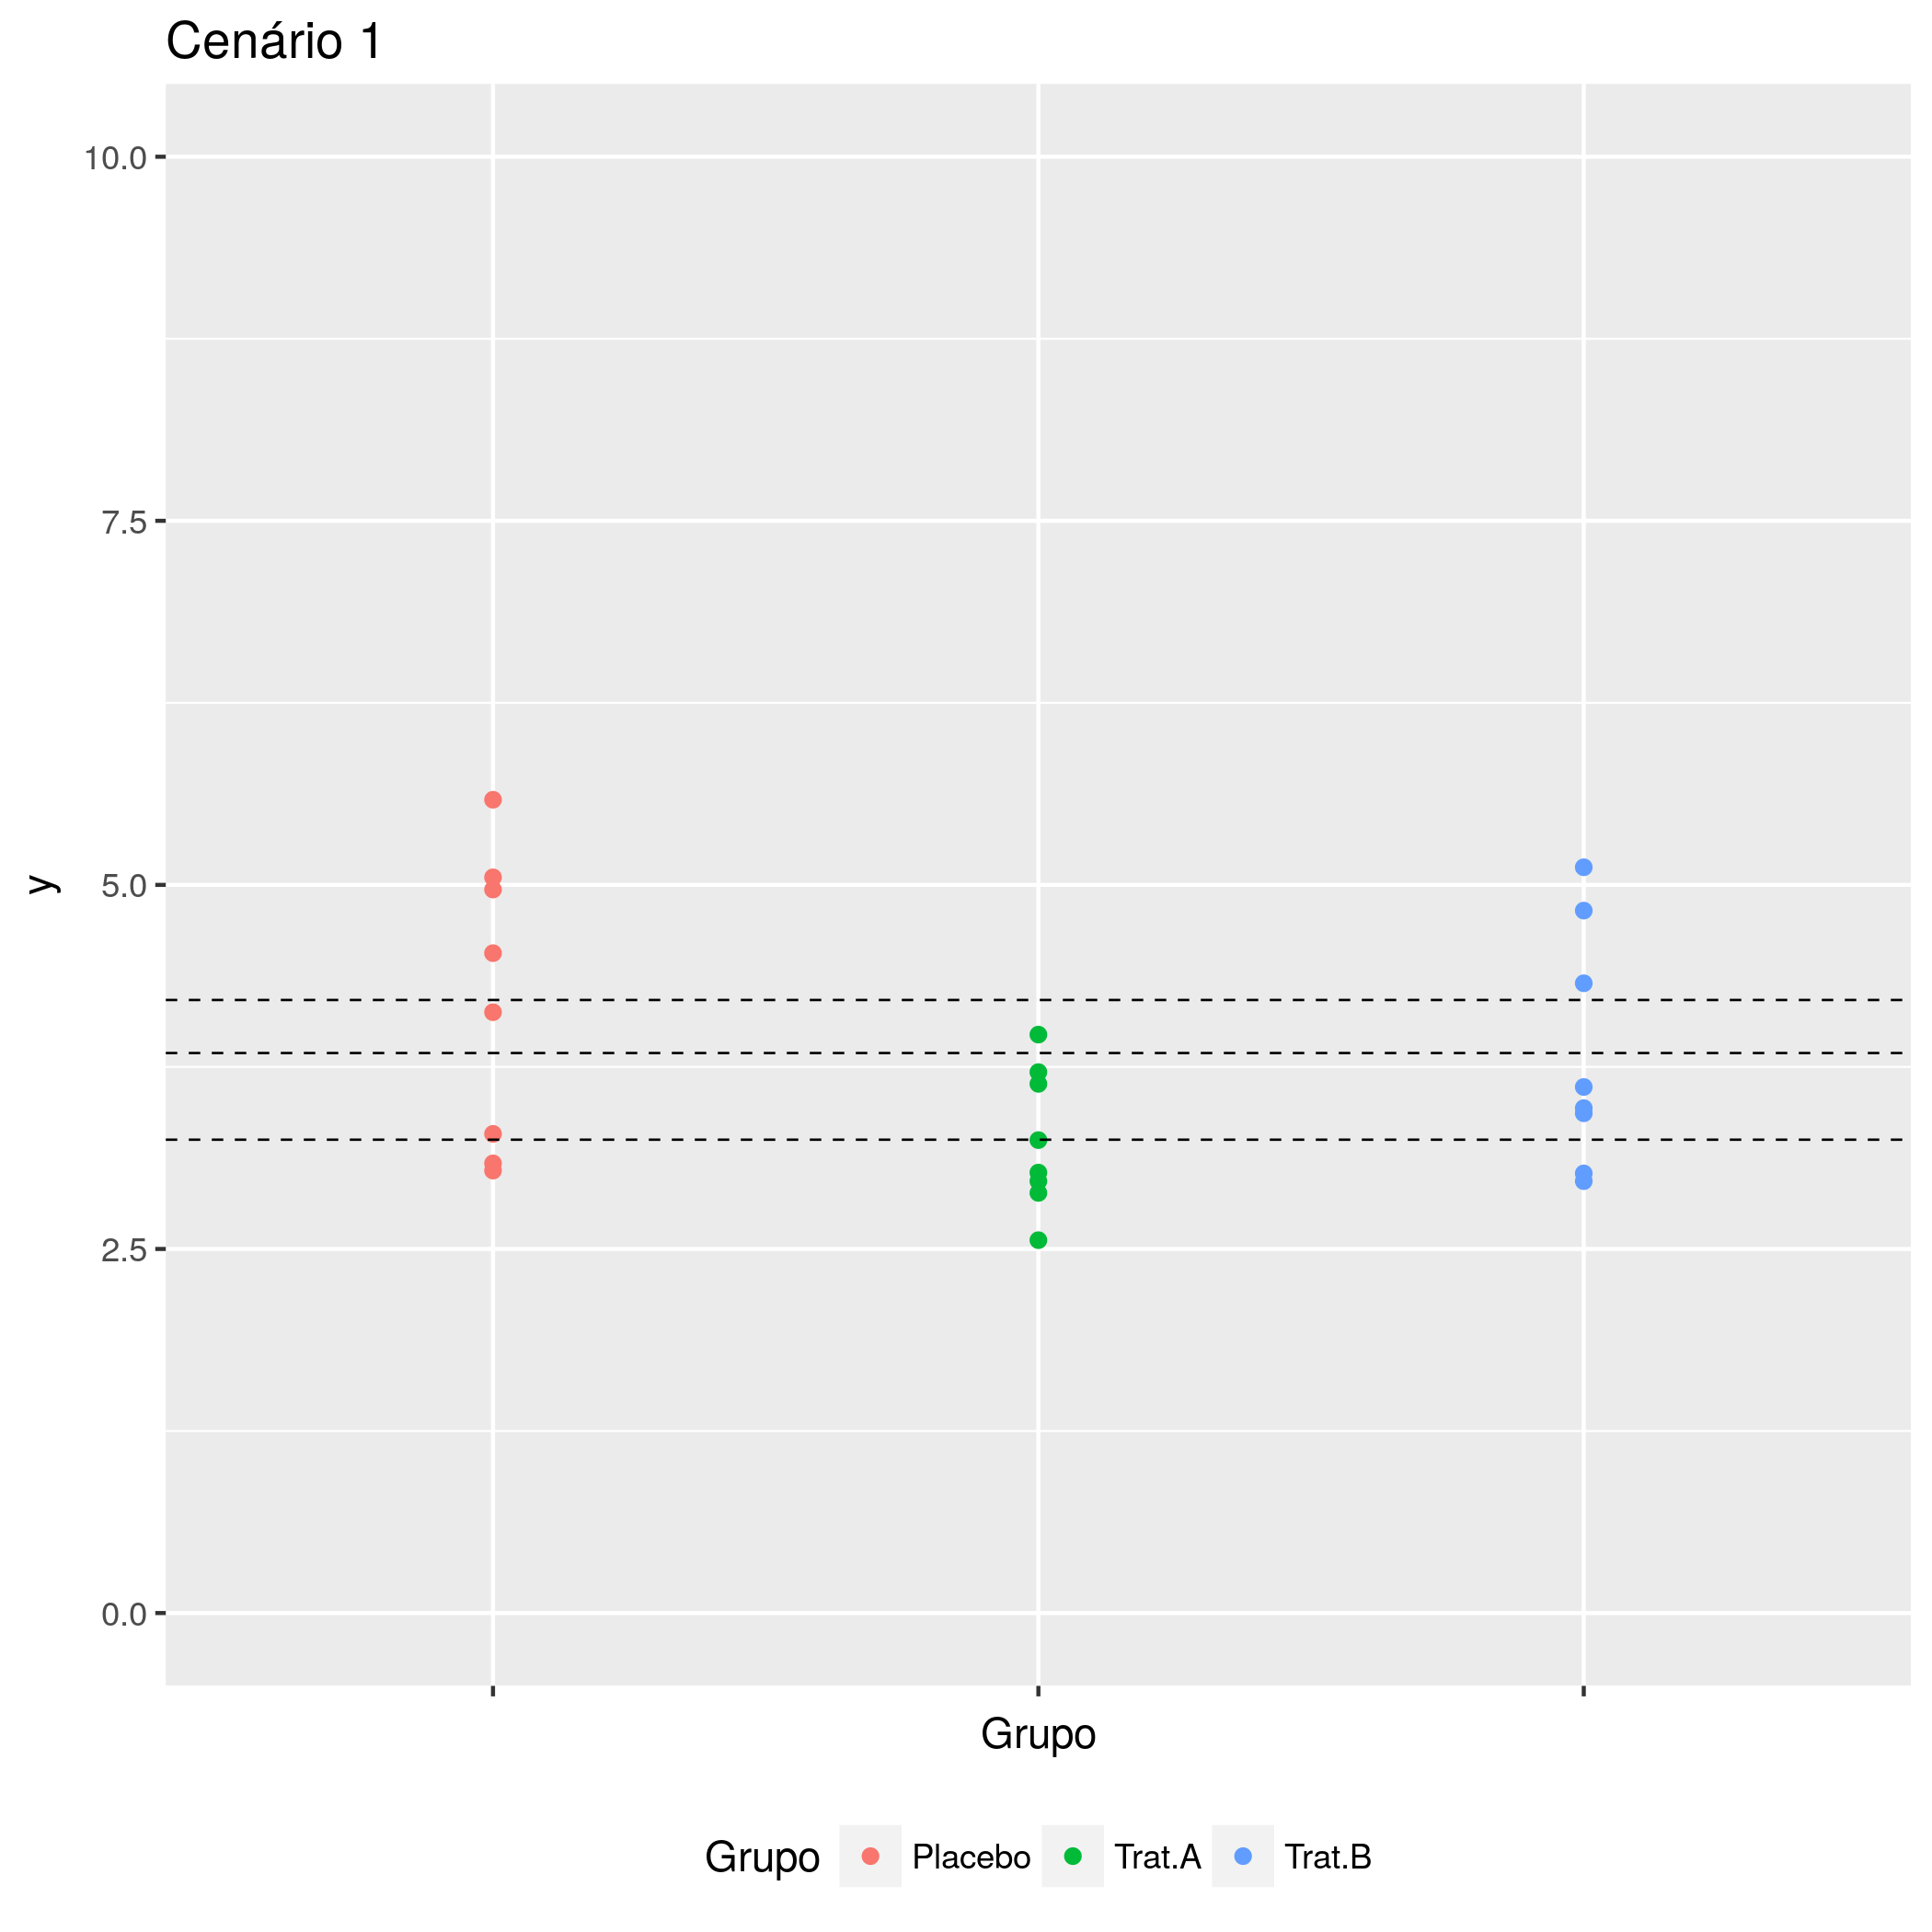
\includegraphics[height=.9\textheight]{Topicos_adv/cenario1_medias}

% %    {\tiny Médias: Placebo: 4.210, Tratamento A: 3.250, Tratamento B: 3.845}
%   \end{center}
% \end{frame}

% \begin{frame}{3 grupos - cenário 2}
%   \begin{center}
%     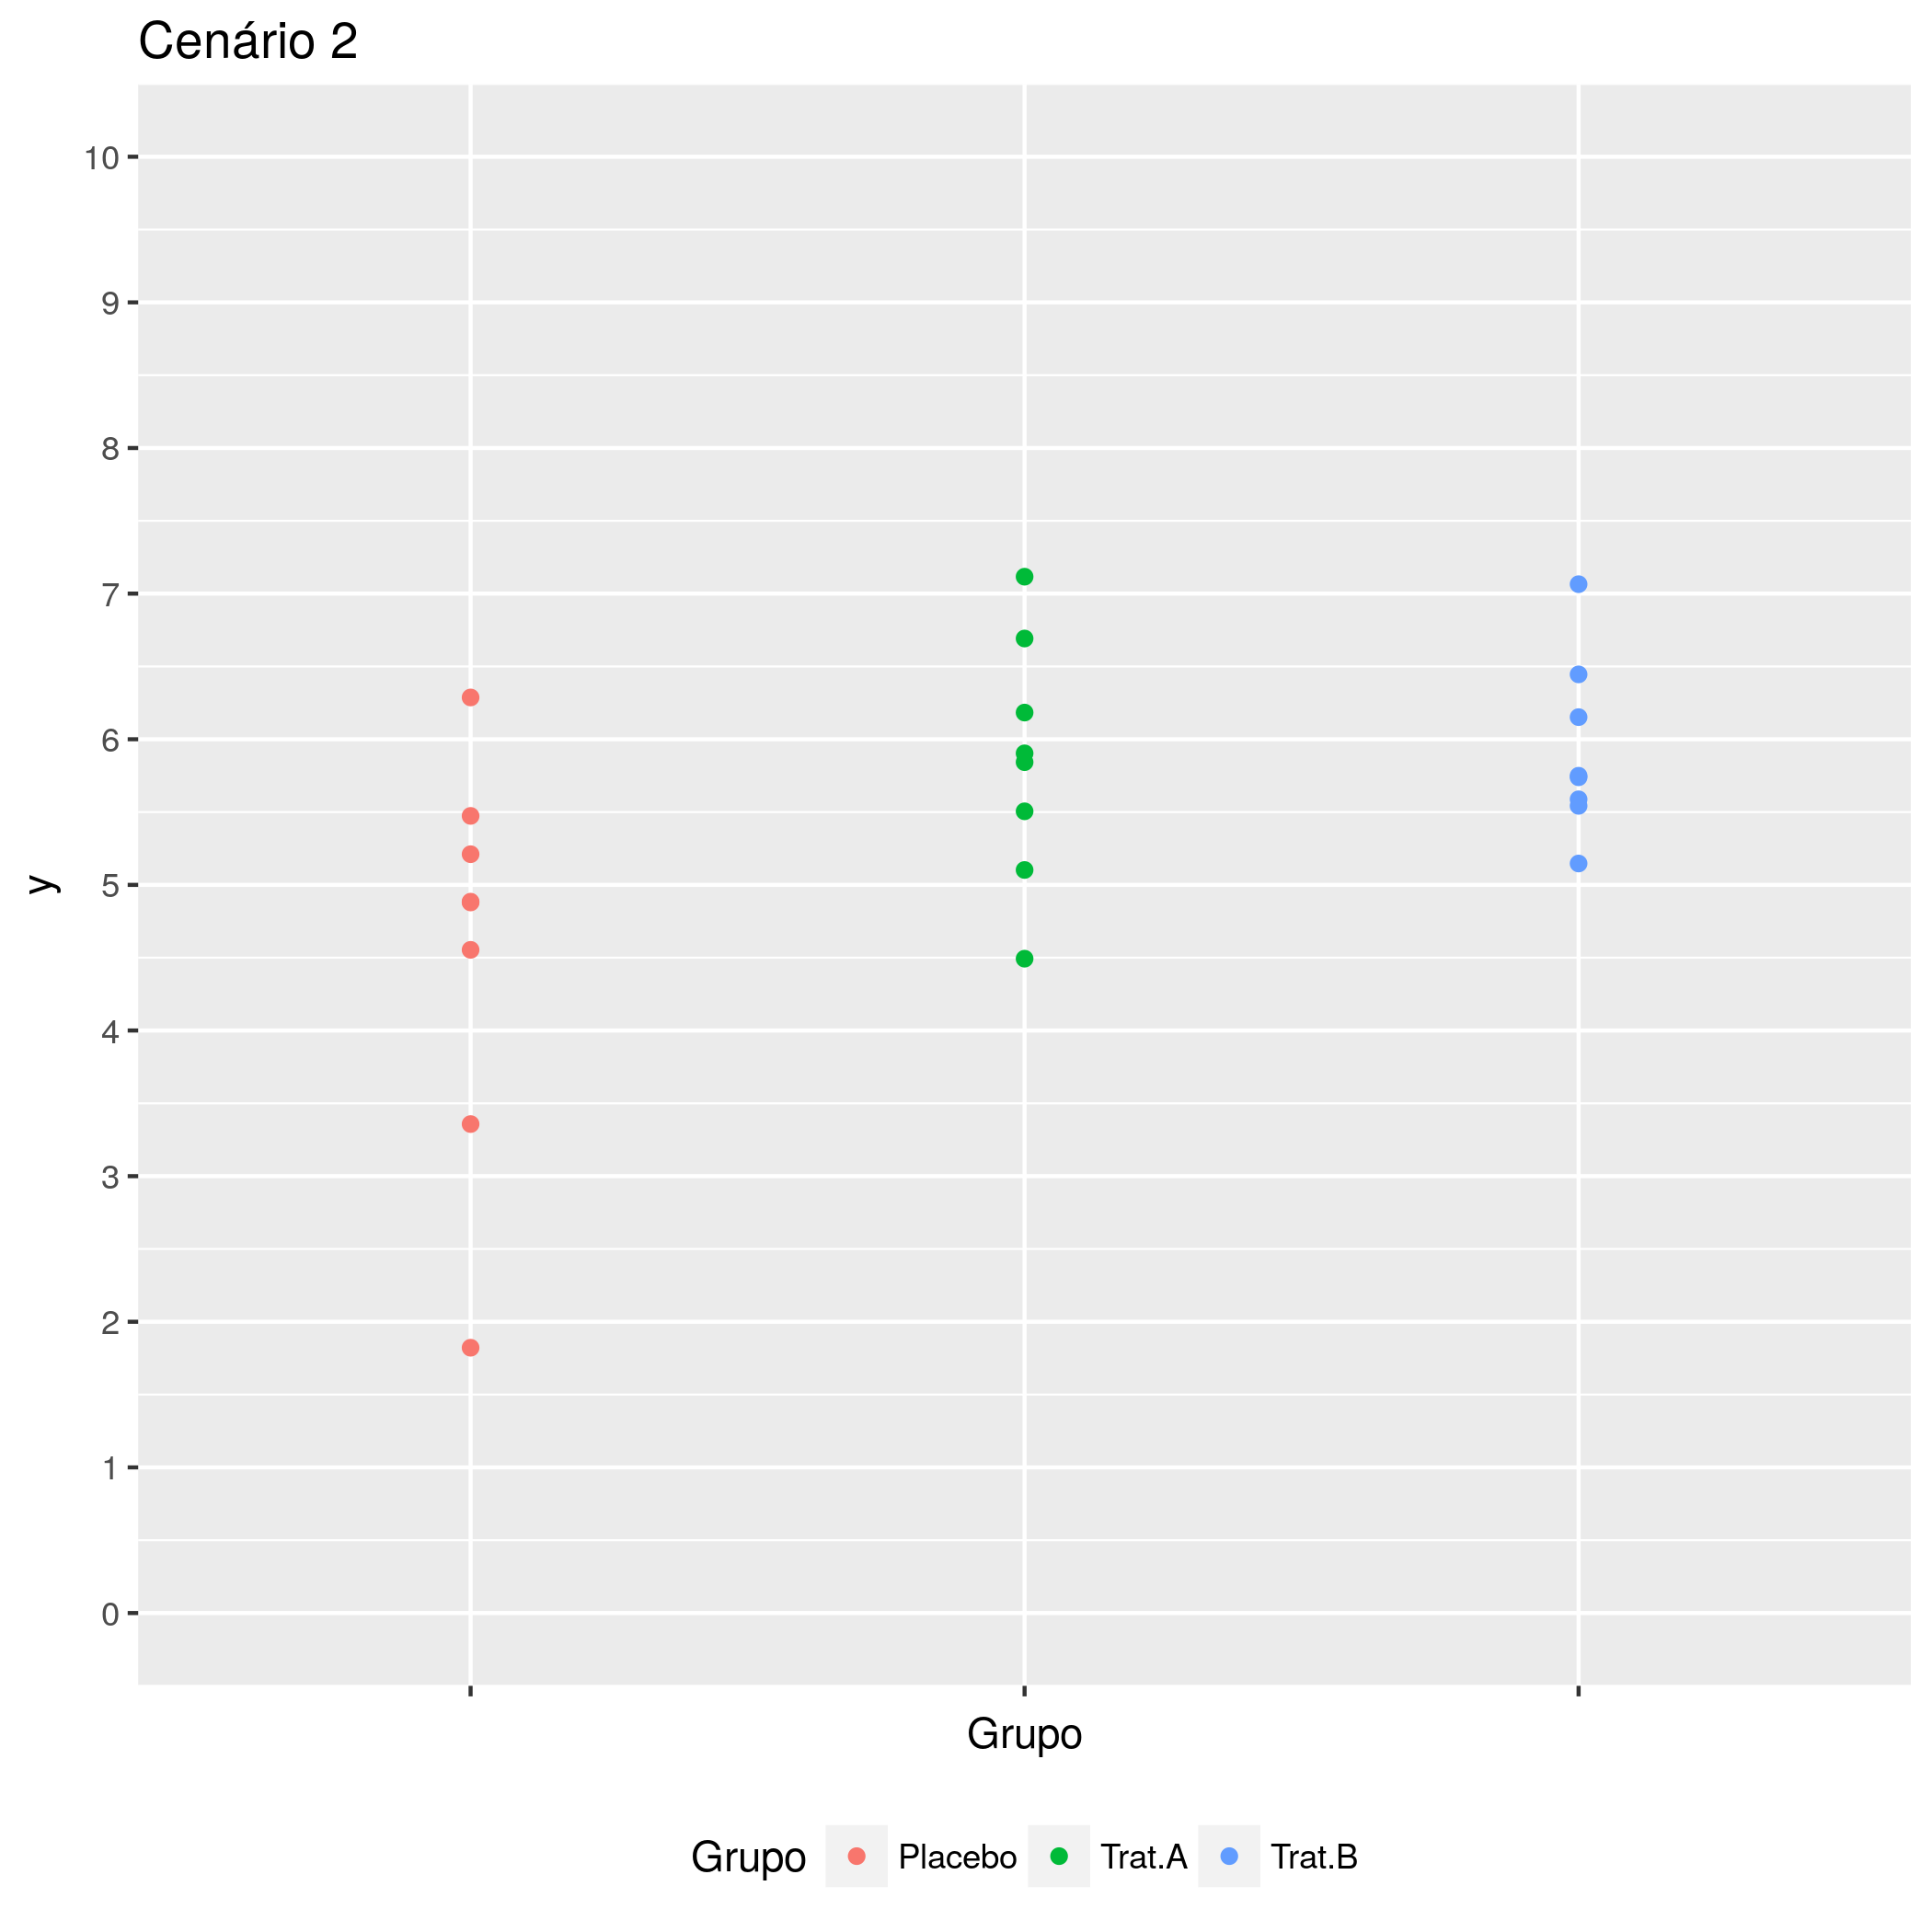
\includegraphics[height=.9\textheight]{Topicos_adv/cenario2}
%   \end{center}
% \end{frame}

% \begin{frame}{Médias: Placebo: 4.559, Tratamento A: 5.855, Tratamento B: 5.928}
%   \begin{center}
%     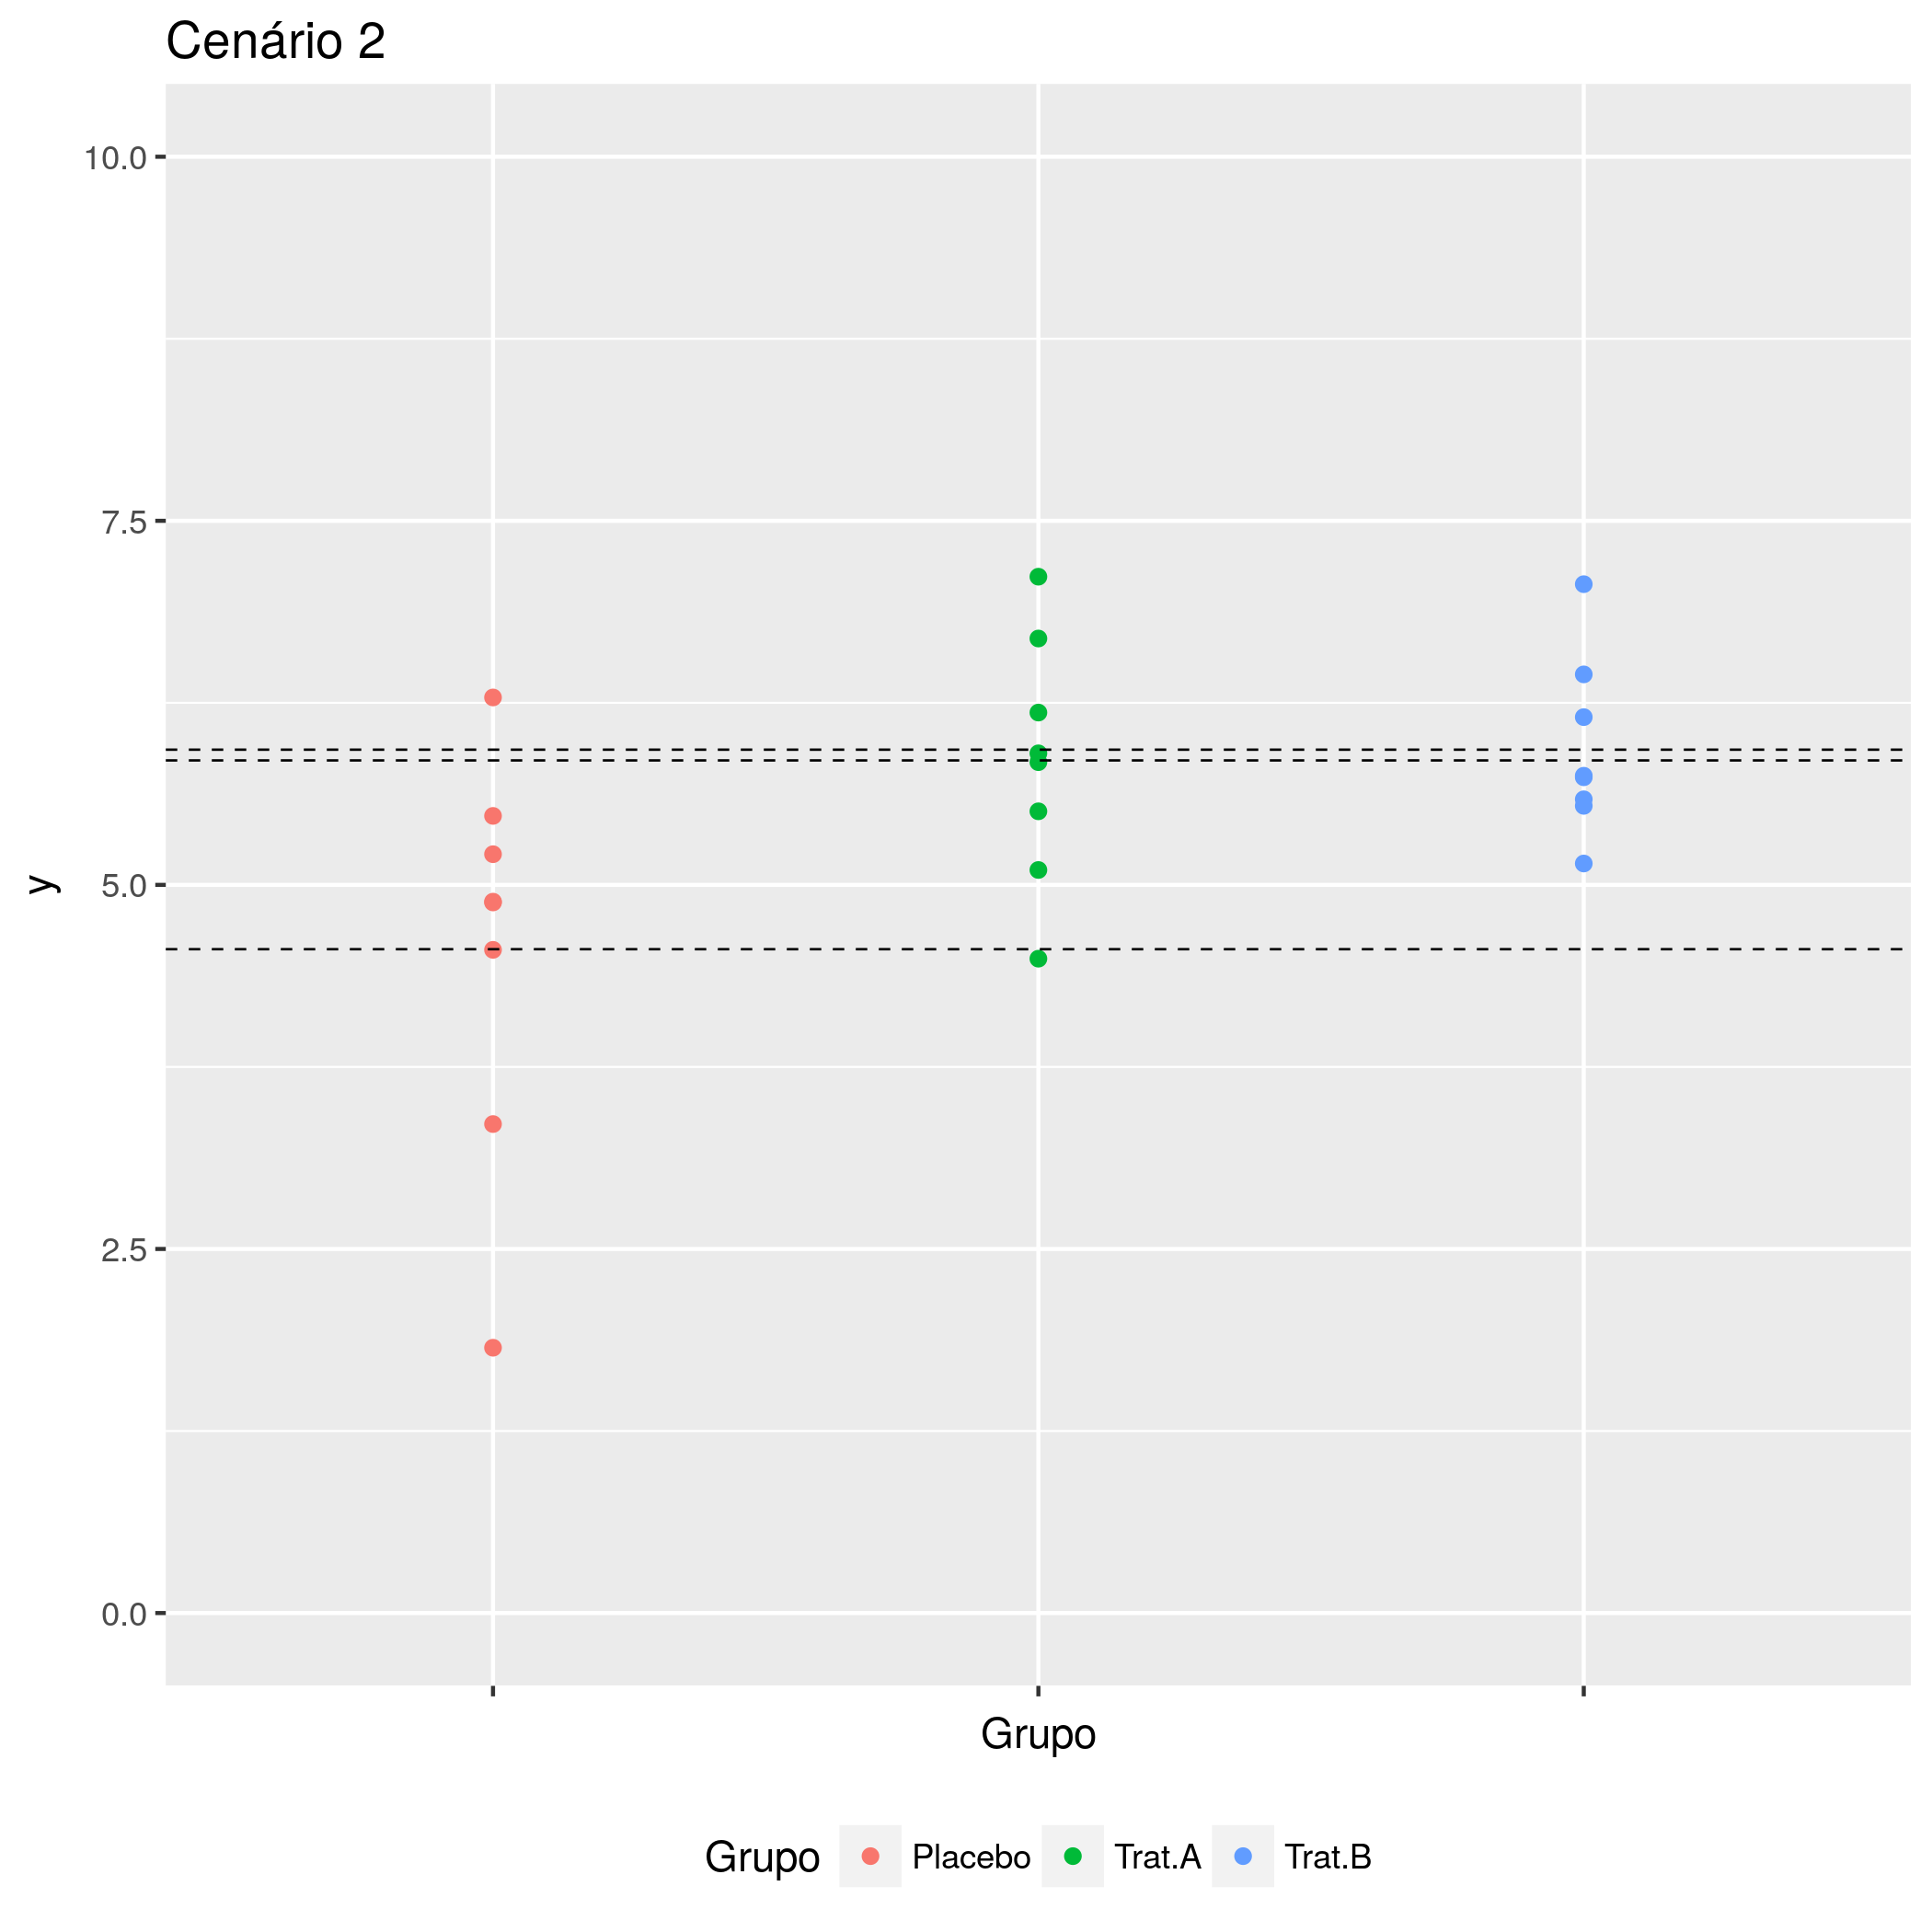
\includegraphics[height=.9\textheight]{Topicos_adv/cenario2_medias}

% %    {\tiny Médias: Placebo: 4.559, Tratamento A: 5.855, Tratamento B: 5.928}
%   \end{center}
% \end{frame}

\subsection{O teste F}

\begin{frame}{O teste F}
  \begin{itemize}
  \item Se as médias forem iguais, a variância intra-grupo deve ser ``igual'' à variância inter-grupo
  \item Calculando-se a {\em razão} entre a variância, esperamos que seja próximo de 1
  \item razão = $F = \frac{\text{Entre grupos}}{\text{Intra grupos}}$
  \item Uma razão muito maior que 1 indica que há mais variância entre os grupos do que o esperado
  \item Obs: o teste leva em conta os graus de liberdade do numerador e denominador
  \end{itemize}
\end{frame}

\begin{frame}{Exemplo}
  \begin{exampleblock}{Exemplo 13.5}
    \begin{center}
      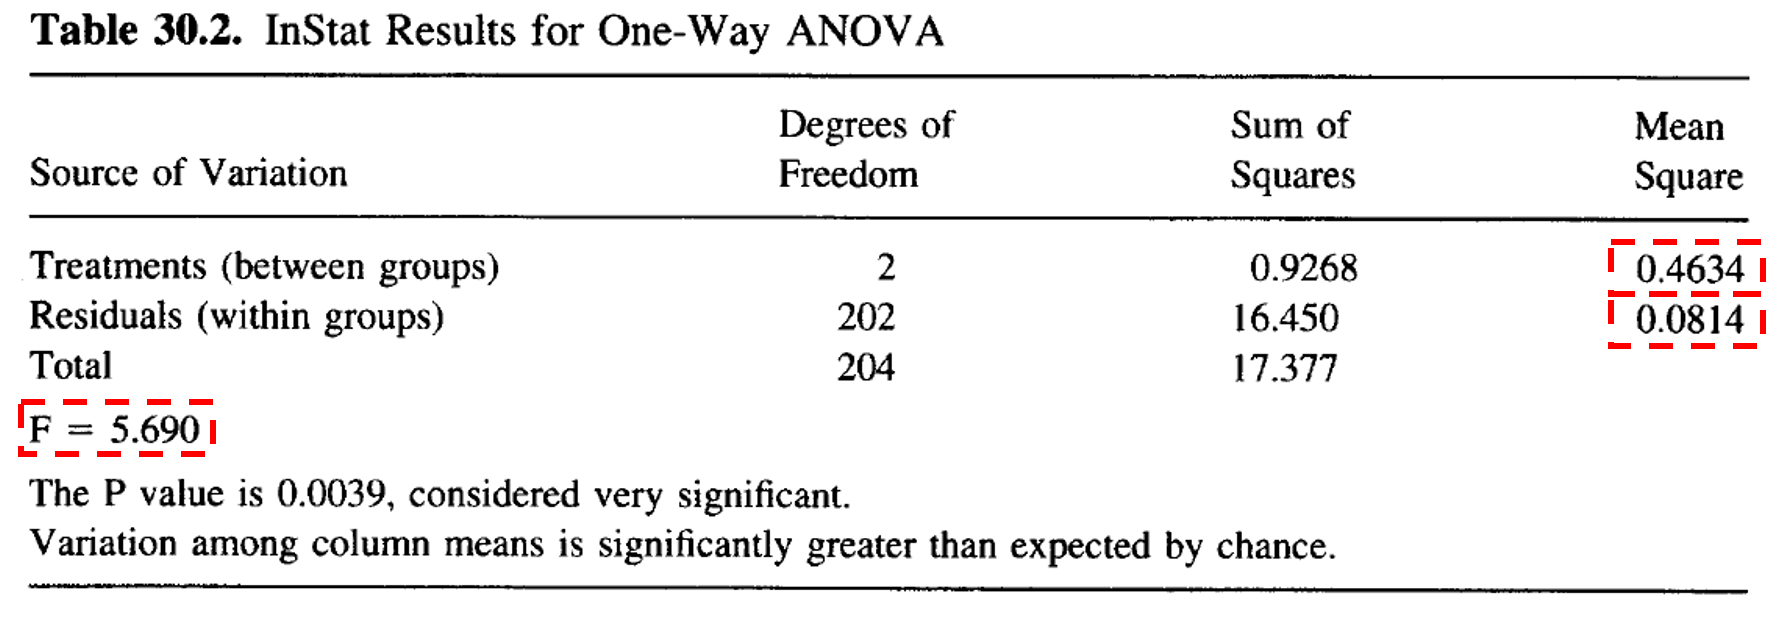
\includegraphics[width=.6\textwidth]{Topicos_adv/exemplo13_5-3}
    \end{center}
  \begin{itemize}
  \item Razão entre as variâncias: $F = 0.4634/0.0814 = 5.69 >> 1$ {\tiny (mesmo considerando o $n$ de cada grupo)}
  \item $p=0.0039$
  \item Pergunta:  Como você redigiria este resultado?
  \end{itemize}
  \end{exampleblock}
\end{frame}

\begin{frame}{}
  \begin{block}{Resposta}
    Sabemos apenas que pelo menos um dos grupos é diferente dos outros.
    Mas qual(is)?

    \bigskip
    Ainda não estamos prontos para redigir o resultado!
  \end{block}
\end{frame}

\subsection{Pós teste}

\begin{frame}{Testes {\em post-hoc}}
  \begin{itemize}
  \item O teste de ANOVA é apenas a primeira parte!\footnote{Está com saudade do teste t?}
  \item O p-valor do teste F indica o quão raro é encontrar uma discrepância tão grande (ou maior) entre as médias dos grupos, ao acaso
  \item Mas isso não nos ajuda a saber qual grupo é diferente dos outros.
  \item Para esta outra pergunta, precisamos de outro método
  \end{itemize}
\end{frame}

\begin{frame}{Testes {\em post-hoc}}
  \begin{itemize}
  \item Como vimos, não podemos simplesmente fazer vários testes t
  \item Mas podemos {\em ajustar} os p-valores destes testes, para compensar a {\em inflação} destes resultados
  \item Isso pode ser feito de várias maneiras
  \end{itemize}
\end{frame}

\begin{frame}{Testes {\em post-hoc}}
  \begin{itemize}
  \item {\bf Correção de Bonferroni}
  \item Correção para tendências
  \item {\bf Teste ``honesto'' das diferenças, de Tukey (HSD)}
  \item Método de Scheffe
  \item Teste de Dunnet
  \end{itemize}
\end{frame}

\begin{frame}{Testes {\em post-hoc}}
  \begin{itemize}
  \item Os dois mais usados são Bonferroni e Tukey
%  \item O teste de Bonferroni é mais simples, e tem mais sensibilidade (com menos especificidade)
%  \item O teste de Tukey tem mais especificidade, mas menos sensibilidade
 \item O teste de Bonferroni ajusta o p-valor dividindo pelo número de comparações, mas seus ICs são muito grandes
 \item O teste de Tukey é mais conservador, mas pode acusar diferenças significativas com mais frequência
 \item Infelizmente não há consenso sobre critérios de escolha
  \end{itemize}
\end{frame}

\begin{frame}{Exemplo}
  \begin{exampleblock}{Exemplo 13.5}
    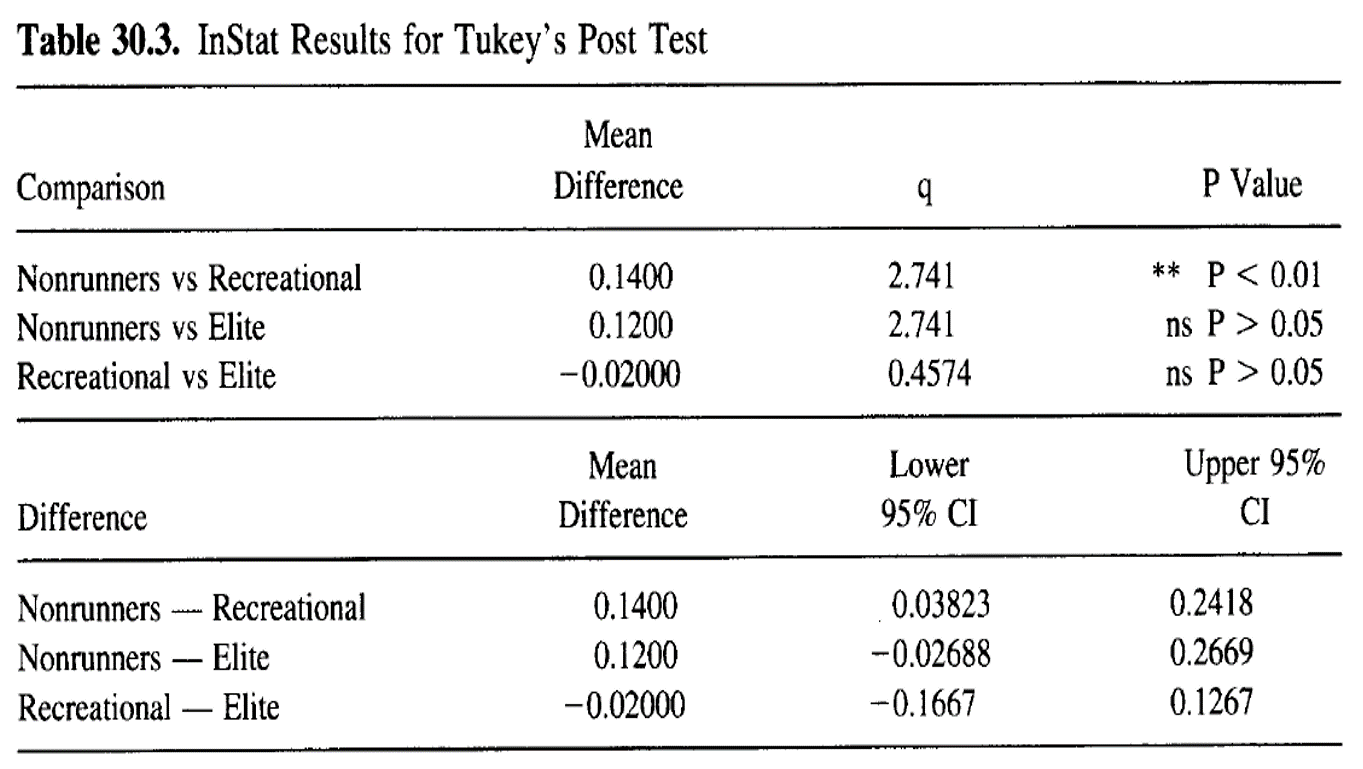
\includegraphics[width=\textwidth]{Topicos_adv/exemplo13_5-4}
  \end{exampleblock}
\end{frame}

\subsection{Two-way ANOVA}

\section{Encerramento}

% \subsection{Resumo}

% \begin{frame}{Resumo}
%   \begin{itemize}
%   \item
%   \end{itemize}
% \end{frame}

\begin{frame}{Leitura pós-aula e exercícios selecionados}
  \begin{block}{Leitura obrigatória}
    \begin{itemize}
    \item Capítulo 13
    \item Capítulo 30
    \end{itemize}
  \end{block}
  \begin{block}{Exercícios}
    Capítulo 13, problema: 1
  \end{block}
  % \begin{block}{Leitura recomendada}
  % \end{block}
\end{frame}

\end{document}
